        %%******************************************%%
        %%                                          %%
        %%        Modello di tesi di laurea         %%
        %%            di Andrea Giraldin            %%
        %%                                          %%
        %%             2 novembre 2012              %%
        %%                                          %%
        %%******************************************%%


% I seguenti commenti speciali impostano:
% 1. 
% 2. PDFLaTeX come motore di composizione;
% 3. tesi.tex come documento principale;
% 4. il controllo ortografico italiano per l'editor.

% !TEX encoding = UTF-8
% !TEX TS-program = pdflatex
% !TEX root = tesi.tex
% !TEX spellcheck = it-IT

% PDF/A filecontents 
\RequirePackage{filecontents}
\begin{filecontents*}{\jobname.xmpdata}
  \Title{Realizzazione di un engine di monitoraggio delle segnalazioni per la notifica di violazioni dei service level agreement}
  \Author{Sinigaglia Alberto}
  \Language{it-IT}
  \Subject{Realizzazione di un engine di monitoraggio delle segnalazioni per la notifica di violazioni dei service level agreement}
  \Keywords{Service Level Agreement\sep Redmine\sep Quality Assurence\sep Rest API \sep Notification System}
\end{filecontents*}

\documentclass[10pt,                    % corpo del font principale
               a4paper,                 % carta A4
               twoside,                 % impagina per fronte-retro
               openright,               % inizio capitoli a destra
               english,                 
               italian,                 
               ]{book}    

%**************************************************************
% Importazione package
%************************************************************** 
\usepackage[table, dvipsnames]{xcolor}
\definecolor{red}{rgb}{0.6,0,0}
\definecolor{blue}{rgb}{0,0,0.6}
\definecolor{green}{rgb}{0,0.8,0}
\definecolor{cyan}{rgb}{0.0,0.6,0.6}
\definecolor{footer-gray}{HTML}{808080}
\definecolor{light-gray}{gray}{0.6} 
\definecolor{light-grayer}{gray}{0.75} 
\definecolor{lighter-grayer}{gray}{0.85} 
\definecolor{lightest-grayest}{gray}{0.94} 
\definecolor{codegreen}{rgb}{0,0.4,0.2}
\definecolor{codegray}{rgb}{0.5,0.5,0.5}
\definecolor{codepurple}{rgb}{0.58,0,0.82}
\definecolor{backcolour}{rgb}{0.95,0.95,0.96}


\PassOptionsToPackage{dvipsnames}{xcolor} % colori PDF/A

\usepackage{colorprofiles}

\usepackage[a-2b,mathxmp]{pdfx}[2018/12/22]
                                        % configurazione PDF/A
                                        % validare in https://www.pdf-online.com/osa/validate.aspx

%\usepackage{amsmath,amssymb,amsthm}    % matematica

\usepackage[T1]{fontenc}                % codifica dei font:
                                        % NOTA BENE! richiede una distribuzione *completa* di LaTeX

\usepackage[utf8]{inputenc}             % codifica di input; anche [latin1] va bene
                                        % NOTA BENE! va accordata con le preferenze dell'editor

\usepackage[english, italian]{babel}    % per scrivere in italiano e in inglese;
                                        % l'ultima lingua (l'italiano) risulta predefinita

\usepackage{bookmark}                   % segnalibri

\usepackage{caption}                    % didascalie

\usepackage{chngpage,calc}              % centra il frontespizio

\usepackage{csquotes}                   % gestisce automaticamente i caratteri (")

\usepackage{emptypage}                  % pagine vuote senza testatina e piede di pagina

\usepackage{epigraph}			% per epigrafi

\usepackage{eurosym}                    % simbolo dell'euro

%\usepackage{indentfirst}               % rientra il primo paragrafo di ogni sezione

\usepackage{graphicx}                   % immagini

\usepackage{hyperref}                   % collegamenti ipertestuali

\usepackage[binding=5mm]{layaureo}      % margini ottimizzati per l'A4; rilegatura di 5 mm

\usepackage{listings}                   % codici

\usepackage{microtype}                  % microtipografia

\usepackage{mparhack,fixltx2e,relsize}  % finezze tipografiche

\usepackage{nameref}                    % visualizza nome dei riferimenti                                      
\usepackage[font=small]{quoting}        % citazioni

\usepackage{subfig}                     % sottofigure, sottotabelle

\usepackage[italian]{varioref}          % riferimenti completi della pagina

\usepackage{booktabs}                   % tabelle                                       
\usepackage{tabularx}                   % tabelle di larghezza prefissata                                    
\usepackage{longtable}                  % tabelle su più pagine                                        
\usepackage{ltxtable}                   % tabelle su più pagine e adattabili in larghezza

\usepackage[toc, acronym]{glossaries}   % glossario
                                        % per includerlo nel documento bisogna:
                                        % 1. compilare una prima volta tesi.tex;
                                        % 2. eseguire: makeindex -s tesi.ist -t tesi.glg -o tesi.gls tesi.glo
                                        % 3. eseguire: makeindex -s tesi.ist -t tesi.alg -o tesi.acr tesi.acn
                                        % 4. compilare due volte tesi.tex.

\usepackage[backend=biber,style=verbose-ibid,hyperref,backref]{biblatex}
                                        % eccellente pacchetto per la bibliografia; 
                                        % produce uno stile di citazione autore-anno; 
                                        % lo stile "numeric-comp" produce riferimenti numerici
                                        % per includerlo nel documento bisogna:
                                        % 1. compilare una prima volta tesi.tex;
                                        % 2. eseguire: biber tesi
                                        % 3. compilare ancora tesi.tex.

\usepackage{multirow,tabularx}
\usepackage{geometry}
\geometry{
	margin=2.0in,
	top=30mm, % NON TOCCARE
	bottom=30mm,
	left=30mm,
	right=35mm
}


%**************************************************************
% file contenente le impostazioni della tesi
%**************************************************************

%**************************************************************
% Frontespizio
%**************************************************************

% Autore
\newcommand{\myName}{Alberto Sinigaglia}     
\newcommand{\myMatr}{1193384}                                    
\newcommand{\myTitle}{Realizzazione di un engine di monitoraggio delle segnalazioni per la notifica di violazioni dei service level agreement}

% Tipo di tesi                   
\newcommand{\myDegree}{Tesi di laurea}

% Università             
\newcommand{\myUni}{Università degli Studi di Padova}

% Facoltà       
\newcommand{\myFaculty}{Corso di Laurea in Informatica}

% Dipartimento
\newcommand{\myDepartment}{Dipartimento di Matematica "Tullio Levi-Civita"}

% Titolo del relatore
\newcommand{\profTitle}{Professoressa }

% Relatore
\newcommand{\myProf}{Gaggi Ombretta}

% Luogo
\newcommand{\myLocation}{Padova}

% Anno accademico
\newcommand{\myAA}{2020-2021}

% Data discussione
\newcommand{\myTime}{Luglio 2021}


%**************************************************************
% Impostazioni di impaginazione
% see: http://wwwcdf.pd.infn.it/AppuntiLinux/a2547.htm
%**************************************************************

\setlength{\parindent}{14pt}   % larghezza rientro della prima riga
\setlength{\parskip}{0pt}   % distanza tra i paragrafi


%**************************************************************
% Impostazioni di biblatex
%**************************************************************
\bibliography{bibliografia} % database di biblatex 

\defbibheading{bibliography} {
    \cleardoublepage
    \phantomsection 
    \addcontentsline{toc}{chapter}{\bibname}
    \chapter*{\bibname\markboth{\bibname}{\bibname}}
}

\setlength\bibitemsep{1.5\itemsep} % spazio tra entry

\DeclareBibliographyCategory{opere}
\DeclareBibliographyCategory{web}

\addtocategory{opere}{womak:lean-thinking}
\addtocategory{web}{site:agile-manifesto}

\defbibheading{opere}{\section*{Riferimenti bibliografici}}
\defbibheading{web}{\section*{Siti Web consultati}}


%**************************************************************
% Impostazioni di caption
%**************************************************************
\captionsetup{
    tableposition=top,
    figureposition=bottom,
    font=small,
    format=hang,
    labelfont=bf
}

%**************************************************************
% Impostazioni di glossaries
%**************************************************************

\setcounter{secnumdepth}{0} % No section number
\setcounter{tocdepth}{0} % No section number


\chapter{Glossario}

\setcounter{secnumdepth}{1} % No section number
\setcounter{tocdepth}{3} % No section number
\subsection{A}
\subsubsection{API}
Interfaccia di programmazione delle applicazioni, che mira a spiegare come utilizzare il servizio dall'esterno (nel nostro caso, è un API web).
\subsubsection{API key}
Metodo di autenticazione ad un API esterna tramite una key univoca fornita dal servizio target.
\subsection{C}
\subsubsection{Customer}
Con Customers ci si riferisce ai clienti, in particolare ai "progetti" aperti sotto il macroprogetto "Customers" dentro Redmine al momento dell'analisi dei requisiti.
\subsection{I}
\subsubsection{Issue}
Guarda "Ticket".
\subsection{R}
\subsubsection{Redmine}
Software utilizzato internamente a Euronovate per la gestione di progetti e ticket.
\subsection{S}
\subsubsection{S.L.A.}
Guarda "Service Level Agreement".
\subsubsection{Service Level Agreement}
Sono strumenti contrattuali attraverso i quali si definiscono le metriche di servizio (nel nostro caso per esempio il tempo massimo di risoluzione di un ticket, o il tempo massimo di presa in carico).

\subsection{T}
\subsubsection{Telegram}
Servizio di messaggistica istantanea (preso in considerazione dal progetto come potenziale mezzo di notifica).
\subsubsection{Ticket}
Sinonimo di Issue, si intende una qualsiasi segnalazione aperta da parte di un Cusotmer. % database di termini
\makeglossaries


%**************************************************************
% Impostazioni di graphicx
%**************************************************************
\graphicspath{{immagini/}} % cartella dove sono riposte le immagini


%**************************************************************
% Impostazioni di hyperref
%**************************************************************
\hypersetup{
    %hyperfootnotes=false,
    %pdfpagelabels,
    %draft,	% = elimina tutti i link (utile per stampe in bianco e nero)
    colorlinks=true,
    linktocpage=true,
    pdfstartpage=1,
    pdfstartview=,
    % decommenta la riga seguente per avere link in nero (per esempio per la stampa in bianco e nero)
    %colorlinks=false, linktocpage=false, pdfborder={0 0 0}, pdfstartpage=1, pdfstartview=FitV,
    breaklinks=true,
    pdfpagemode=UseNone,
    pageanchor=true,
    pdfpagemode=UseOutlines,
    plainpages=false,
    bookmarksnumbered,
    bookmarksopen=true,
    bookmarksopenlevel=1,
    hypertexnames=true,
    pdfhighlight=/O,
    %nesting=true,
    %frenchlinks,
    urlcolor=webbrown,
    linkcolor=RoyalBlue,
    citecolor=webgreen,
    %pagecolor=RoyalBlue,
    %urlcolor=Black, linkcolor=Black, citecolor=Black, %pagecolor=Black,
    pdftitle={\myTitle},
    pdfauthor={\textcopyright\ \myName, \myUni, \myFaculty},
    pdfsubject={},
    pdfkeywords={},
    pdfcreator={pdfLaTeX},
    pdfproducer={LaTeX}
}

%**************************************************************
% Impostazioni di itemize
%**************************************************************
\renewcommand{\labelitemi}{$\ast$}

%\renewcommand{\labelitemi}{$\bullet$}
%\renewcommand{\labelitemii}{$\cdot$}
%\renewcommand{\labelitemiii}{$\diamond$}
%\renewcommand{\labelitemiv}{$\ast$}


%**************************************************************
% Impostazioni di listings
%**************************************************************
\lstset{
    language=[LaTeX]Tex,%C++,
    keywordstyle=\color{RoyalBlue}, %\bfseries,
    basicstyle=\small\ttfamily,
    %identifierstyle=\color{NavyBlue},
    commentstyle=\color{Green}\ttfamily,
    stringstyle=\rmfamily,
    numbers=none, %left,%
    numberstyle=\scriptsize, %\tiny
    stepnumber=5,
    numbersep=8pt,
    showstringspaces=false,
    breaklines=true,
    frameround=ftff,
    frame=single
} 


%**************************************************************
% Impostazioni di xcolor
%**************************************************************
\definecolor{webgreen}{rgb}{0,.5,0}
\definecolor{webbrown}{rgb}{.6,0,0}


%**************************************************************
% Altro
%**************************************************************

\newcommand{\omissis}{[\dots\negthinspace]} % produce [...]

% eccezioni all'algoritmo di sillabazione
\hyphenation
{
    ma-cro-istru-zio-ne
    gi-ral-din
}

\newcommand{\sectionname}{sezione}
\addto\captionsitalian{\renewcommand{\figurename}{Figura}
                       \renewcommand{\tablename}{Tabella}}

\newcommand{\glsfirstoccur}{\ap{{[g]}}}

\newcommand{\intro}[1]{\emph{\textsf{#1}}}

%**************************************************************
% Environment per ``rischi''
%**************************************************************
\newcounter{riskcounter}                % define a counter
\setcounter{riskcounter}{0}             % set the counter to some initial value

%%%% Parameters
% #1: Title
\newenvironment{risk}[1]{
    \refstepcounter{riskcounter}        % increment counter
    \par \noindent                      % start new paragraph
    \textbf{\arabic{riskcounter}. #1}   % display the title before the 
                                        % content of the environment is displayed 
}{
    \par\medskip
}

\newcommand{\riskname}{Rischio}

\newcommand{\riskdescription}[1]{\textbf{\\Descrizione:} #1.}

\newcommand{\risksolution}[1]{\textbf{\\Soluzione:} #1.}

%**************************************************************
% Environment per ``use case''
%**************************************************************
\newcounter{usecasecounter}             % define a counter
\setcounter{usecasecounter}{0}          % set the counter to some initial value

%%%% Parameters
% #1: ID
% #2: Nome
\newenvironment{usecase}[2]{
    \renewcommand{\theusecasecounter}{\usecasename #1}  % this is where the display of 
                                                        % the counter is overwritten/modified
    \refstepcounter{usecasecounter}             % increment counter
    \vspace{10pt}
    \par \noindent                              % start new paragraph
    {\large \textbf{\usecasename #1: #2}}       % display the title before the 
                                                % content of the environment is displayed 
    \medskip
}{
    \medskip
}

\newcommand{\usecasename}{UC}

\newcommand{\usecaseactors}[1]{\textbf{\\Attori Principali:} #1. \vspace{4pt}}
\newcommand{\usecasepre}[1]{\textbf{\\Precondizioni:} #1. \vspace{4pt}}
\newcommand{\usecasedesc}[1]{\textbf{\\Descrizione:} #1. \vspace{4pt}}
\newcommand{\usecasepost}[1]{\textbf{\\Postcondizioni:} #1. \vspace{4pt}}
\newcommand{\usecasealt}[1]{\textbf{\\Scenario Alternativo:} #1. \vspace{4pt}}

%**************************************************************
% Environment per ``namespace description''
%**************************************************************

\newenvironment{namespacedesc}{
    \vspace{10pt}
    \par \noindent                              % start new paragraph
    \begin{description} 
}{
    \end{description}
    \medskip
}

\newcommand{\classdesc}[2]{\item[\textbf{#1:}] #2}


                     % file con le impostazioni personali
\newcommand{\gloxy}[1]{\emph{#1}$_G$}
\setlength{\tabcolsep}{10pt}
\renewcommand{\arraystretch}{1.4}
\usepackage{hyperref}
\hypersetup{
	colorlinks,
	citecolor=black,
	filecolor=black,
	linkcolor=black,
	urlcolor=black
}


\begin{document}
%**************************************************************
% Materiale iniziale
%**************************************************************
\frontmatter
% !TEX encoding = UTF-8
% !TEX TS-program = pdflatex
% !TEX root = ../tesi.tex

%**************************************************************
% Frontespizio 
%**************************************************************
\begin{titlepage}

\begin{center}

\begin{LARGE}
\textbf{\myUni}\\
\end{LARGE}

\vspace{10pt}

\begin{Large}
\textsc{\myDepartment}\\
\end{Large}

\vspace{10pt}

\begin{large}
\textsc{\myFaculty}\\
\end{large}

\vspace{30pt}
\begin{figure}[htbp]
\begin{center}

\includegraphics[height=6cm]{logo-unipd}
\end{center}
\end{figure}
\vspace{30pt} 

\begin{LARGE}
\begin{center}
\textbf{\myTitle}\\
\end{center}
\end{LARGE}

\vspace{10pt} 

\begin{large}
\textsl{\myDegree}\\
\end{large}

\vspace{30pt} 

\begin{large}
\begin{flushleft}
\textit{Relatore}\\ 
\vspace{5pt} 
\profTitle \myProf
\end{flushleft}

\vspace{0pt} 

\begin{flushright}
\textit{Laureando}\\ 
\vspace{5pt} 
\myName
\end{flushright}
\end{large}

\vspace{30pt}

\line(1, 0){338} \\
\begin{normalsize}
\textsc{Anno Accademico \myAA}
\end{normalsize}

\end{center}
\end{titlepage} 
% !TEX encoding = UTF-8
% !TEX TS-program = pdflatex
% !TEX root = ../tesi.tex

%**************************************************************
% Colophon
%**************************************************************
\clearpage
\phantomsection
\thispagestyle{empty}

\hfill

\vfill

\noindent\myName: \textit{\myTitle,}
\myDegree,
\textcopyright\ \myTime.
% !TEX encoding = UTF-8
% !TEX TS-program = pdflatex
% !TEX root = ../tesi.tex

%**************************************************************
% Dedica
%**************************************************************
\cleardoublepage
\phantomsection
% !TEX encoding = UTF-8
% !TEX TS-program = pdflatex
% !TEX root = ../tesi.tex

%**************************************************************
% Sommario
%**************************************************************
\cleardoublepage
\phantomsection
\pdfbookmark{Sommario}{Sommario}
\begingroup
\let\clearpage\relax
\let\cleardoublepage\relax
\let\cleardoublepage\relax

\chapter*{Sommario}

Il presente documento descrive il lavoro svolto durante il periodo di stage, della durata di circa trecento ore, dal laureando Alberto Sinigaglia presso l'azienda EsignWorld.\\
Lo stage aveva come obiettivo l'analisi e lo sviluppo di un sistema di monitoraggio delle segnalazioni, per la verifica e la notifica di potenziali violazioni delle S.L.A. stipulate con i clienti.\\
Il sistema in questione aveva come requisiti:
\begin{enumerate}
	\item interfacciarsi con il portale per la segnalazione di problemi utilizzato in azienda (Redmine)
	\item esser modulare, così da permettere una migrazione ad altri sistemi di segnalazione
	\item notificare tramite diversi canali potenziali violazioni delle S.L.A.
\end{enumerate}
Per far ciò è stata eseguita inizialmente una fase di studio dei componenti, seguita dall'analisi dei requisiti, per poi concludersi nello sviluppo del prodotto, che in conclusione ha portato alla demo finale.

%\vfill
%
%\selectlanguage{english}
%\pdfbookmark{Abstract}{Abstract}
%\chapter*{Abstract}
%
%\selectlanguage{italian}

\endgroup			

\vfill


% !TEX encoding = UTF-8
% !TEX TS-program = pdflatex
% !TEX root = ../tesi.tex

%**************************************************************
% Ringraziamenti
%**************************************************************
\cleardoublepage
\phantomsection
\pdfbookmark{Ringraziamenti}{ringraziamenti}

\begin{flushright}{
	\slshape    
	``Not everything that counts can be counted, \\and not everything that can be counted counts.''} \\ 
	\medskip
    --- Albert Einstein
\end{flushright}


\bigskip

\begingroup
\let\clearpage\relax
%\let\cleardoublepage\relax
\let\cleardoublepage\relax

\chapter*{Ringraziamenti}

\# TODO

\noindent \textit{Innanzitutto, vorrei esprimere la mia gratitudine alla Professoressa Gaggi Ombretta, relatore della mia tesi, per l'aiuto e il sostegno fornitomi durante la stesura del lavoro.}\\

\noindent \textit{Desidero ringraziare con affetto i miei genitori e annessi compagni per il sostegno, il grande aiuto e per essermi stati vicini in ogni momento durante gli anni di studio.}\\

\bigskip

\noindent\textit{\myLocation, \myTime}
\hfill \myName

\endgroup


% !TEX encoding = UTF-8
% !TEX TS-program = pdflatex
% !TEX root = ../tesi.tex

%**************************************************************
% Indici
%**************************************************************
\cleardoublepage
\pdfbookmark{\contentsname}{tableofcontents}
\setcounter{tocdepth}{2}
\tableofcontents
%\markboth{\contentsname}{\contentsname} 
\clearpage

\begingroup 
    \let\clearpage\relax
    \let\cleardoublepage\relax
    \let\cleardoublepage\relax
    %*******************************************************
    % Elenco delle figure
    %*******************************************************    
    \phantomsection
    \pdfbookmark{\listfigurename}{lof}
    \listoffigures

    \vspace*{8ex}

    %*******************************************************
    % Elenco delle tabelle
    %*******************************************************
    \phantomsection
    \pdfbookmark{\listtablename}{lot}
    \listoftables
        
    \vspace*{8ex}
\endgroup

\cleardoublepage

\cleardoublepage

%**************************************************************
% Materiale principale
%**************************************************************
\mainmatter
% !TEX encoding = UTF-8
% !TEX TS-program = pdflatex
% !TEX root = ../tesi.tex

%**************************************************************
\chapter{Introduzione}
\label{cap:introduzione}
%**************************************************************

Il seguente capitolo vuole introdurre brevemente il progetto affrontato e l'azienda ospitante ideatrice di esso. \\



\iffalse
\noindent Esempio di utilizzo di un termine nel glossario \\
\gls{api}. \\
\noindent Esempio di citazione in linea \\
\cite{site:agile-manifesto}. \\
\noindent Esempio di citazione nel pie' di pagina \\
citazione\footcite{womak:lean-thinking} \\
\fi


%**************************************************************
\section{L'azienda}

\par EsignWorld è un'azienda italiana facente parte del gruppo Euronovate, gruppo del settore IT che conta circa 120 collaboratori, con sede centrale in Svizzera con varie sedi in Spagna, Italia, Romania e Cina. 
\newline
\newline
\par EsignWorld si occupa di sviluppare e progettare soluzioni complesse nell'ambito della digital identity, digital signature e digital onboarding, sia software che hardware riguardanti i processi di dematerializzazione all'interno delle aziende.
\newline
\newline
\par Durante lo stage ci si è andati ad interfacciare con Redmine, che per quanto non sia un prodotto sviluppato direttamente da Euronovate, è utilizzato internamente per la pianificazione di progetti e per il tracciamento delle segnalazioni di bug.
\newline
\begin{figure}[!h] 
	\centering 
	
\includegraphics[width=0.5\columnwidth]{logo-azienda.png} 
	\caption{Logo dell'azienda}
\end{figure}
\begin{figure}[!h] 
	\centering 
	
\includegraphics[width=0.5\columnwidth]{logo-redmine.png} 
	\caption{Logo di Redmine}
\end{figure}

%**************************************************************
\section{L'idea}

Lo stage consiste nello sviluppo di un prodotto software per il monitoraggio delle segnalazioni, con conseguente notifica in caso di violazioni dei service level agreement stipulati tra l'azienda e i clienti.\\
Per raggiungere tale obiettivo, ci si è appoggiati a Redmine, software adottato dall'azienda per la gestione delle segnalazioni e l'ottenimento dei dati necessari alle analisi. Redmine infatti raccoglie tutti i dati fondamentali, quali segnalazioni, tempo dedicato per ogni task e un log di tutti i cambiamenti avvenuti. \\
Il prodotto periodicamente quindi scarica gli aggiornamenti da Redmine, li analizza, e tramite delle policy predefinite per ogni cliente, va a notificare tramite vari canali l'eventuale violazione di esse. \\
Infine, l'applicativo espone un'API per l'ottenimento di informazioni statistiche riguardanti le violazioni. 

%**************************************************************
\section{Organizzazione del testo}

\begin{description}
    \item[{\hyperref[cap:processi-metodologie]{Il secondo capitolo}}] espone una panoramica sugli obbiettivi dello stage e la sua pianificazione, con un'analisi preventiva dei rischi.
    
    \item[{\hyperref[cap:descrizione-stage]{Il terzo capitolo}}] descrive l'analisi dei requisiti del progetto affrontato nello stage, durante la quale son state definite le funzionalità desiderate.
    
    \item[{\hyperref[cap:analisi-requisiti]{Il quarto capitolo}}] approfondisce ...
    
    \item[{\hyperref[cap:progettazione-codifica]{Il quinto capitolo}}] approfondisce ...
    
    \item[{\hyperref[cap:verifica-validazione]{Il sesto capitolo}}] approfondisce ...
    
    \item[{\hyperref[cap:conclusioni]{Nel settimo capitolo}}] descrive ...
\end{description}

Riguardo la stesura del testo, relativamente al documento sono state adottate le seguenti convenzioni tipografiche:
\begin{itemize}
	\item gli acronimi, le abbreviazioni e i termini ambigui o di uso non comune menzionati vengono definiti nel glossario, situato alla fine del presente documento;
	\item per la prima occorrenza dei termini riportati nel glossario viene utilizzata la seguente nomenclatura: \gloxy{parola};
	\item i termini in lingua straniera o facenti parti del gergo tecnico sono evidenziati con il carattere \emph{corsivo}.
\end{itemize}             % Introduzione
\iffalse % !TEX encoding = UTF-8
% !TEX TS-program = pdflatex
% !TEX root = ../tesi.tex

%**************************************************************
\chapter{Processi e metodologie}
\label{cap:processi-metodologie}
%**************************************************************

\intro{Brevissima introduzione al capitolo}\\

%**************************************************************
\section{Processo sviluppo prodotto}      \fi       % Processi 
% !TEX encoding = UTF-8
% !TEX TS-program = pdflatex
% !TEX root = ../tesi.tex

%**************************************************************
\chapter{Descrizione dello stage}
\label{cap:descrizione-stage}
%**************************************************************

\intro{In questa sezione verrà trattato come si è svolto lo stage presso EsignWorld, considerando gli obiettivi pianificati, discutendo dei possibili rischi e la comunicazione con il tutor aziendale.}\\

\section{Introduzione}
Lo stage presso EsignWorld aveva come scopo la creazione di un engine che monitorasse i ticket aperti dai clienti dell'azienda per capire se si fosse in procinto di violare le Service Level Agreement stipulate con tale cliente. \\
Per far ciò, ci si è andati a interfacciare a Redmine, prodotto usato internamente dall'azienda per la gestione di progetti e l'apertura di ticket. Grazie ad esso quindi, ci si è potuti sollevare la parte di gestione del ticket e dei clienti, focalizzandosi solo sulla parte di analisi e notifica. \\
Una volta ottenuti i dati da Redmine, l'engine doveva appunto analizzare i dati, confrontarli con le S.L.A. fornitegli per ogni cliente, e in caso si fosse vicini al violarle, o la violazione fosse già avvenuta, procedere a segnalarlo al responsabile, tramite molteplici canali di notifica (quali per esempio Telegram e Email). \\
Infine, il progetto doveva predisporre anche un API per la pubblicazione dei dati: tale API aveva come scopo un monitoraggio statistico dei ticket, delle segnalazioni e delle violazioni, e quindi mirava a preparare i dati per esempio per graficarli o manipolarli.


%**************************************************************
\section{Obiettivi del progetto}
\begin{itemize}
	\item Principali:
	\begin{enumerate}
		\item Studio e valutazione di componenti esterni ai quali interfacciarsi successivamente.
		\item Test e recupero dati dai servizi esposti da Redmine.
		\item Analisi di vari sistemi di notifica, come Telegram e Email.
		\item Redazione di un documento di Analisi dei Requisiti.
		\item Redazione di un documento di Progettazione Tecnica.
		\item Sviluppo/Codifica del progetto seguendo le norme di codifica aziendali.
		\item Redazione documentazione del progetto:
		\begin{enumerate}
			\item Manuale di manutenzione.
			\item Manuale di installazione.
			\item Documentazione API.
		\end{enumerate}
	\end{enumerate}
	\item Secondari:
	\begin{enumerate}
		\item Integrazione dell'API con l'applicativo ENAnalytics
		\item Integrazione della base di dati con l'applicativo Grafana
		\item Sviluppo di test di unità e di integrità
	\end{enumerate}
\end{itemize}


%**************************************************************
\section{Analisi preventiva dei rischi}

Durante la fase di analisi iniziale sono stati individuati alcuni possibili rischi a cui si poteva andare incontro.
Si è quindi proceduto a elaborare delle possibili soluzioni per far fronte ad essi.\\


\begin{risk}{Tecnologie nuove}
    \riskdescription{le tecnologie consigliate per lo sviluppo del progetto erano nuove, causando un'inevitabile inesperienza nel loro utilizzo}
    \risksolution{è stato predefinito un periodo iniziale di formazione personale per le tecnologie che son state poi utilizzate per lo sviluppo, così da aver tempo di familiarizzarci leggermente e arrivare alla codifica con le nozioni base già apprese}
\end{risk}
\begin{risk}{Sistemi esterni}
	\riskdescription{il progetto richiede di interfacciarsi con sistemi esterni (quali per esempio Redmine) mai usati prima e che potrebbero avere una documentazione non esaustiva}
	\risksolution{è stata predefinito un periodo iniziale di formazione personale sui sistemi ai quali ci si è interfacciati durante la codifica, così da avere già una chiara visione del loro funzionamento e delle feature che mettono a disposizione}
\end{risk}
\begin{risk}{Gestione dello smart working}
	\riskdescription{lo stage si è tenuto interamente da remoto, portando quindi a un potenziale rischio di mancanza di comunicazione, che avrebbe potuto portare a un'incerta comprensione degli obbiettivi dello stage e del progetto affrontato}
	\risksolution{si è deciso di avere un meeting giornaliero con il tutor aziendale nelle prime fasi del progetto, così da esser sicuri che si arrivasse alle fasi finali (come la codifica) con tutti i chiarimenti necessari espletati}
\end{risk}
 


%**************************************************************

\subsection{Pianificazione}
	Di seguito sono elencate le varie fasi previste per lo stage e una loro stima oraria, in ordine cronologico:
	\begin{enumerate}
		\item \textbf{Conoscenze generali}: ($\sim$1 giorno) approfondimento e installazione degli ambienti di sviluppo e di versionamento, e abilitazione strumenti aziendali. 
		\item \textbf{Acquisizione degli standard aziendali}: ($\sim$1 giorno) esposizione dei servizi server Euronovate e dell'architettura della soluzione di firma Euronovate. 
		\item \textbf{Formazione personale}: ($\sim$5 giorni) formazione sul framework target per lo sviluppo, valutazione e test di componenti esterni (sistemi di notifica come email e messaggistica istantanea), istruzione sull'applicativo Redmine e recupero dati dai suoi servizi esposti.
		\item \textbf{Analisi dei requisiti}: ($\sim$4 giorni) analisi del tipo di informazioni da monitorare e successivamente da esporre/pubblicare, selezione dei sistemi e delle regole di notifica (e relativa frequenza di aggiornamento dati locali).
		\item \textbf{Progettazione tecnica}: ($\sim$5 giorni) stesura della specifica tecnica del Back-End, dei servizi esposti e degli oggetti di scambio.
		\item \textbf{Codifica}: ($\sim$18 giorni) sviluppo del prodotto seguendo le norme di codifica aziendali e potenzialmente test di unità e integrità.
		\item \textbf{Documentazione}: ($\sim$4 giorni) stesura manuale di manutenzione, manuale di installazione, e documentazione API.
		\item \textbf{Demo}: ($\sim$1 giorno) presentazione del prodotto sviluppato dall'azienda. 
	\end{enumerate}
	Il tutto può essere visualizzato nel seguente Gantt Chart:
	\begin{center}
		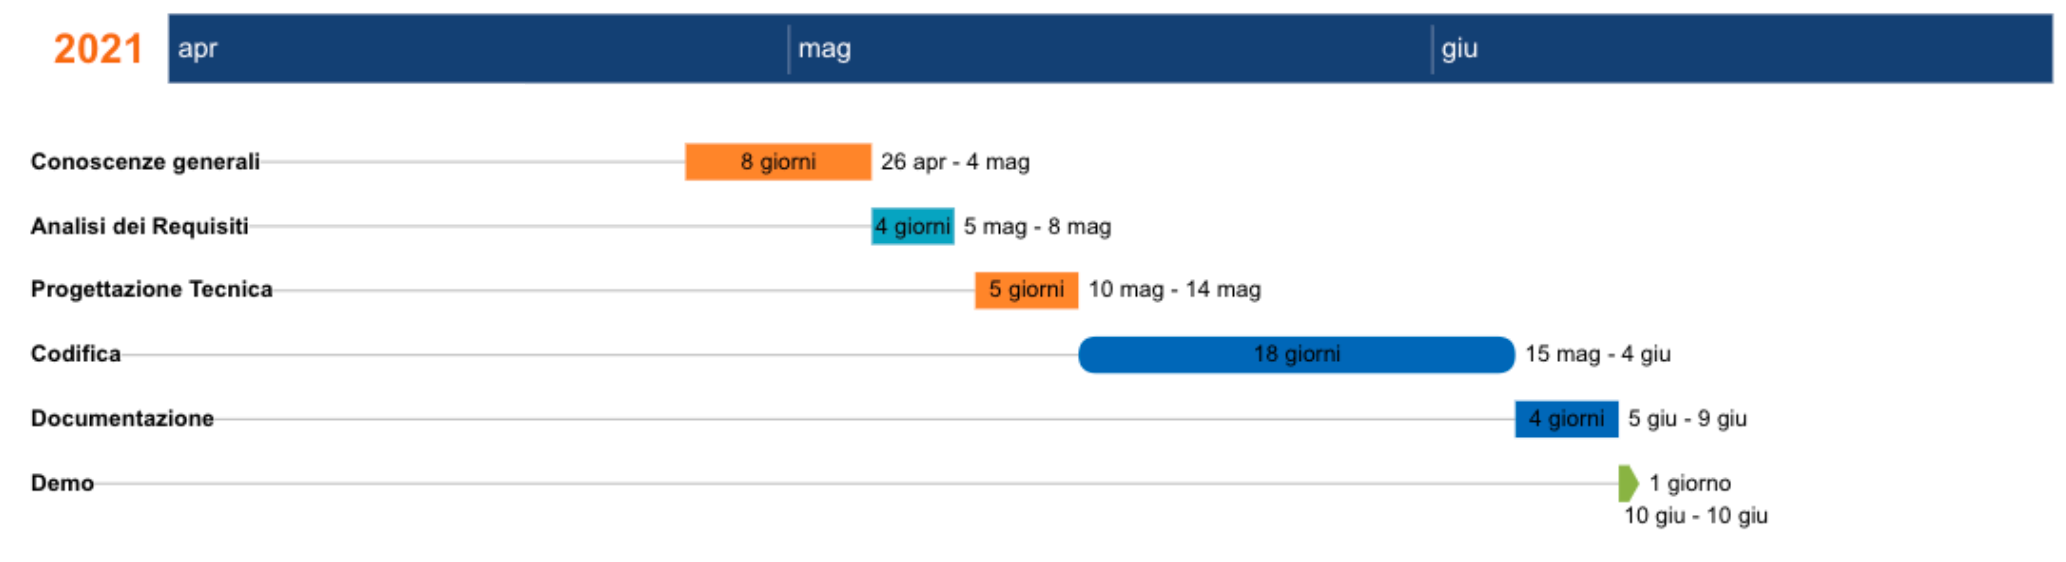
\includegraphics[keepaspectratio = true, width=15cm]{immagini/pianificazione.png}
		\captionof{figure}{Pianificazione dello stage}
	\end{center}
\iffalse
	\subsection{Suddivisione del carico di lavoro}
		\begin{center}
			\begin{table}[h!]
				\centering
				\begin{tabular}{c | c | c | c} 
					\textbf{Fase} & \textbf{Data inizio} & \textbf{Data fine} & \textbf{Durata}\\
					\hline
					Conoscenze generali   & 26/04/2021 & 04/05/2021 & 64 \\
					Analisi dei requisiti       & 05/05/2021 & 08/05/2021 & 32 \\
					Progettazione tecnica & 10/05/2021 & 14/05/2021 & 40 \\
					Codifica                       & 15/05/2021 & 04/06/2021 & 144 \\
					Documentazione         & 05/06/2021 & 09/06/2021 & 32 \\
					Demo                           & 10/06/2021 & 10/06/2021 & 8 \\
					\hline\hline
					\multicolumn{3}{l}{\textbf{Totale}} & 320 \\
				\end{tabular}
				\vspace{0.3cm}
				\caption{Tabella della suddivisione delle ore per ogni fase del progetto di stage}
			\end{table}
		\end{center}
\fi
		             % Kick-Off
% !TEX encoding = UTF-8
% !TEX TS-program = pdflatex
% !TEX root = ../tesi.tex

%**************************************************************
\chapter{Analisi dei requisiti}
\label{cap:analisi-requisiti}
%**************************************************************

\intro{Breve introduzione al capitolo}\\

\section{Casi d'uso}

Per lo studio dei casi di utilizzo del prodotto sono stati creati dei diagrammi.
I diagrammi dei casi d'uso (in inglese \emph{Use Case Diagram}) sono diagrammi di tipo \gls{uml} dedicati alla descrizione delle funzioni o servizi offerti da un sistema, così come sono percepiti e utilizzati dagli attori che interagiscono col sistema stesso.
Essendo il progetto finalizzato alla creazione di un tool per l'automazione di un processo, le interazioni da parte dell'utilizzatore devono essere ovviamente ridotte allo stretto necessario. Per questo motivo i diagrammi d'uso risultano semplici e in numero ridotto.

\begin{figure}[!h] 
    \centering 
    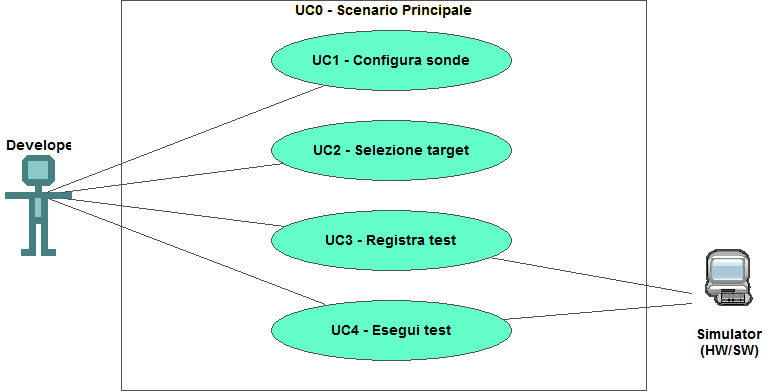
\includegraphics[width=0.9\columnwidth]{usecase/scenario-principale} 
    \caption{Use Case - UC0: Scenario principale}
\end{figure}

\begin{usecase}{0}{Scenario principale}
\usecaseactors{Sviluppatore applicativi}
\usecasepre{Lo sviluppatore è entrato nel plug-in di simulazione all'interno dell'IDE}
\usecasedesc{La finestra di simulazione mette a disposizione i comandi per configurare, registrare o eseguire un test}
\usecasepost{Il sistema è pronto per permettere una nuova interazione}
\label{uc:scenario-principale}
\end{usecase}

\section{Tracciamento dei requisiti}

Da un'attenta analisi dei requisiti e degli use case effettuata sul progetto è stata stilata la tabella che traccia i requisiti in rapporto agli use case.\\
Sono stati individuati diversi tipi di requisiti e si è quindi fatto utilizzo di un codice identificativo per distinguerli.\\
Il codice dei requisiti è così strutturato R(F/Q/V)(N/D/O) dove:
\begin{enumerate}
	\item[R =] requisito
    \item[F =] funzionale
    \item[Q =] qualitativo
    \item[V =] di vincolo
    \item[N =] obbligatorio (necessario)
    \item[D =] desiderabile
    \item[Z =] opzionale
\end{enumerate}
Nelle tabelle \ref{tab:requisiti-funzionali}, \ref{tab:requisiti-qualitativi} e \ref{tab:requisiti-vincolo} sono riassunti i requisiti e il loro tracciamento con gli use case delineati in fase di analisi.

\newpage

\begin{table}%
\caption{Tabella del tracciamento dei requisti funzionali}
\label{tab:requisiti-funzionali}
\begin{tabularx}{\textwidth}{lXl}
\hline\hline
\textbf{Requisito} & \textbf{Descrizione} & \textbf{Use Case}\\
\hline
RFN-1     & L'interfaccia permette di configurare il tipo di sonde del test & UC1 \\
\hline
\end{tabularx}
\end{table}%

\begin{table}%
\caption{Tabella del tracciamento dei requisiti qualitativi}
\label{tab:requisiti-qualitativi}
\begin{tabularx}{\textwidth}{lXl}
\hline\hline
\textbf{Requisito} & \textbf{Descrizione} & \textbf{Use Case}\\
\hline
RQD-1    & Le prestazioni del simulatore hardware deve garantire la giusta esecuzione dei test e non la generazione di falsi negativi & - \\
\hline
\end{tabularx}
\end{table}%

\begin{table}%
\caption{Tabella del tracciamento dei requisiti di vincolo}
\label{tab:requisiti-vincolo}
\begin{tabularx}{\textwidth}{lXl}
\hline\hline
\textbf{Requisito} & \textbf{Descrizione} & \textbf{Use Case}\\
\hline
RVO-1    & La libreria per l'esecuzione dei test automatici deve essere riutilizzabile & - \\
\hline
\end{tabularx}
\end{table}%             % Concept Preview
% !TEX encoding = UTF-8
% !TEX TS-program = pdflatex
% !TEX root = ../tesi.tex

%**************************************************************
\chapter{Progettazione e codifica}
\label{cap:progettazione-codifica}
%**************************************************************

\intro{In questo capitolo viene esposta la progettazione tecnica e la successiva codifica del prodotto ENTicketEngine.}\\


\section{Analisi dell'architettura}
In questa sezione verrà analizzata l'architettura dei vari sistemi richiesti per la realizzazione del progetto \textbf{ENTicketEngine}.\\

    \subsection{Architettura}
        L'architettura del prodotto è riassunta nel diagramma riportato in figura 4.1
        \begin{center}
            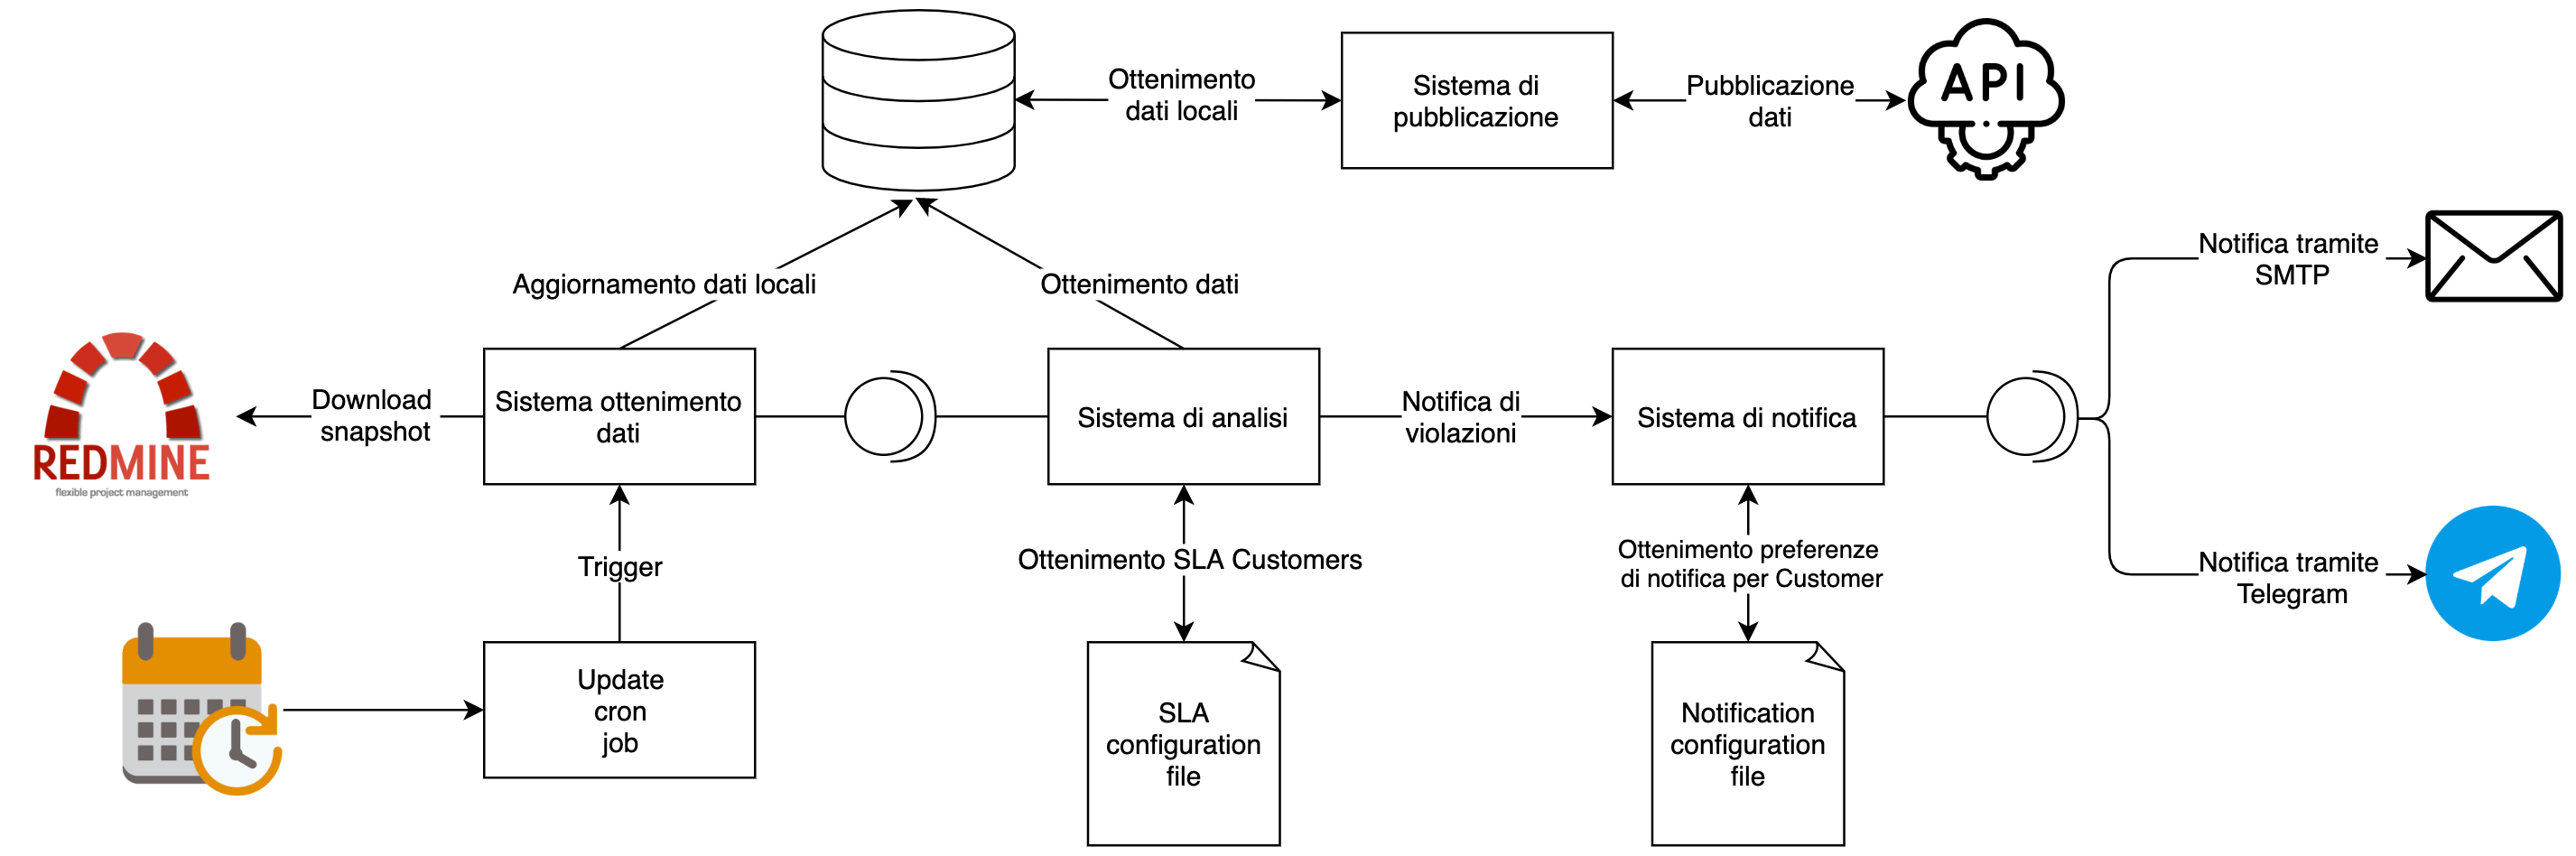
\includegraphics[keepaspectratio = true, width=15cm]{immagini/progettazione/architettura.png}
            \captionof{figure}{Architettura generale del prodotto}
        \end{center}
    	Si possono notare principalmente 3 sistemi che collaborano tra di loro per il raggiungimento dell'obbiettivo, in particolare:
    	\begin{itemize}
    		\item sistema di ottenimento: responsabile del reperimento dei dati dal sistema esterno (in figura rappresentato dal logo Redmine);
    		\item sistema di analisi: responsabile dell'individuazione delle violazioni / segnalazioni da notificare;
    		\item sistema di notifica: responsavile dell'invio delle notifiche ai responsabili  tramite vari canali di notifica (in figura rappresentati dal loro Mail e Telegram);
    		\item sistema di pubblicazione: responsabile dell'esposizione dei dati presenti nella base di dati all'esterno tramite una RESTful API (in figura rappresentata dal logo API).
    	\end{itemize}
    	Tali sistemi sono poi avviati tramite un \texttt{cron-job} per effettuare l'aggiornamento periodicamente.\\
    	Per il corretto funzionamento e per rendere possibile la personalizzazione dei vari parametri, i sistemi si interfacciano a file XML esterni.
        \subsection{Analisi dei sistemi}
            Il prodotto prevede principalmente 4 sistemi: l'\gloxy{API} di pubblicazione, il sistema di ottenimento dei dati, il sistema di analisi, ed infine il sistema di notifica.
        \subsubsection{Sistema ottenimento dati}
            Questo sistema essendo responsabile dell'ottenimento dei dati, si è dovuto appoggiare al servizio esterno scelto (in questo caso, \gloxy{Redmine}) per il raggiungimento del suo scopo. \\
            Da Analisi dei Requisiti risulta un requisito che tale sistema però possa in futuro essere cambiato facilmente: ciò implica che il sistema di ottenimento dati debba essere il più possibile disaccoppiato dal sistema con il quale si andrà a interfacciare. \\
            Per far ciò quindi, si è proceduto a creare un modulo per interfacciarsi al servizio esterno, che è stato accoppiato al sistema di ottenimento dati tramite \texttt{(Object) Adapter design pattern}.
            \begin{quote}
            	\mbox{}%
            	\vspace{-1cm}
                   
                    \subparagraph*{Dipendenze esterne}
                    \mbox{} \\
                        Questo sistema si può scomporre in 2 sottosistemi:
                        \begin{enumerate}
                            \item un sottosistema per ottenere i dati;
                            \item un sottosistema per salvare gli oggetti ottenuti nella base di dati.
                        \end{enumerate}
                        Il tutto è rappresentato nel grafico riportato in figura 4.2
                        \begin{center}
                            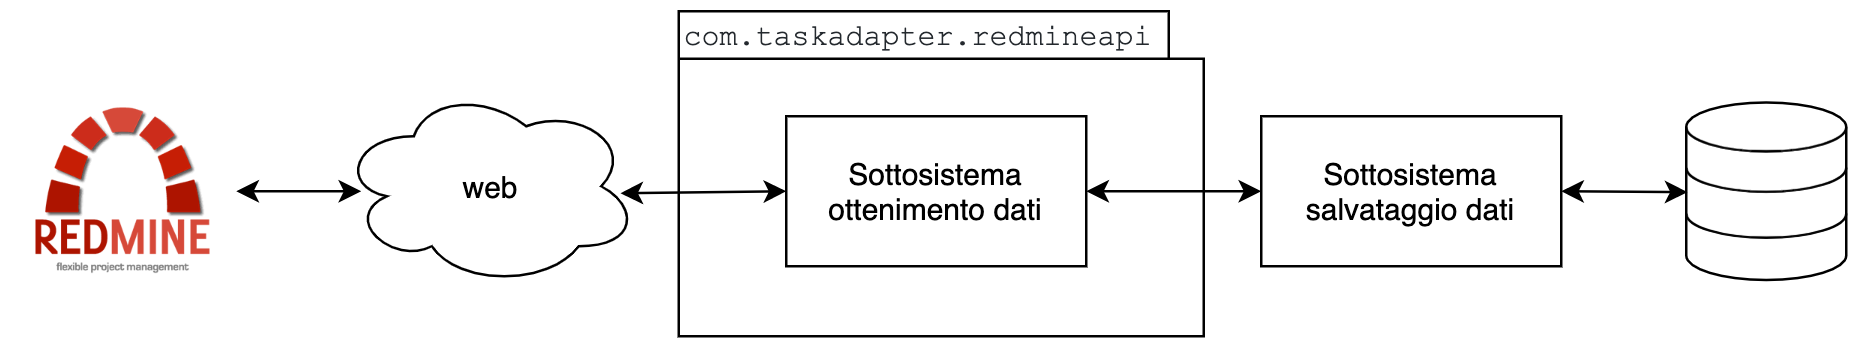
\includegraphics[keepaspectratio = true, width=14cm]{immagini/progettazione/ottenimento.png}
                            \captionof{figure}{Struttura del sistema di ottenimento}
                        \end{center}
                        Come si può notare dal diagramma riportato in figura 4.2, fa uso della dipendenza \texttt{com.taskadapter:redmine-java-api} per andare a interfacciarsi con Redmine.
            \end{quote}
        \subsubsection{Sistema analisi dati}
            Questo sistema essendo responsabile della notifica delle violazioni, doveva prevedere degli algoritmi, che date le configurazioni lette inizialmente, analizzeranno i dati per trovare violazioni o segnalazioni. \\
            Considerato che le necessità e i vincoli potevano cambiare, è stato usato \texttt{Strategy design pattern} per l'algoritmo, e considerato che le configurazioni delle \gloxy{S.L.A.} sono componibili (possono avere o meno una durata massima di presa in carico, possono o meno avere una durata massima di risoluzione, ecc ecc), si poteva far uso di \texttt{Decorator design pattern} per la logo generazione da file, ma durante la fase di codifica ci si è confrontati con il reparto di Quality Assurance che hanno garantico che tali vincoli son presenti per tutti (e se così non fosse, vengono applicati dei vincoli di default).
            \begin{quote}
            	\mbox{}%
            	\vspace{-1cm}
                    \subparagraph{Dipendenze esterne}
                    \mbox{} \\
                        Non sono state identificate dipendenze esterne per questo sistema.
            \end{quote}
        \subsubsection{Sistema di notifica}
            Questo sistema, per raggiungere il suo obiettivo, doveva interfacciarsi con sistemi esterni, per i quali esistono già \gloxy{SDK} completi e testati. \\
            Per permettere la modularità di tale sistema, e la possibilità di integrare nuovi canali di notifica senza andare a modificare codice pre-esistente, si è fatto uso del \texttt{Adapter design pattern} per conformare tutti i canali sotto un unica interfaccia, e nel caso tali SDK non fossero esistiti, si avrebbe fatto uso dell'\texttt{ereditarietà} per la loro creazione.
            \begin{quote}
            	\mbox{}%
            	\vspace{-1cm}
                    
                    \subparagraph{Dipendenze esterne}
                    \mbox{} \\
                        Questo sistema si può scomporre in 2 sottosistemi:
                        \begin{enumerate}
                            \item un sottosistema per la gestione dei canali di notifica;
                            \item un sottosistema per ogni canale di notifica.
                        \end{enumerate}
                        Il tutto è rappresentato nel grafico riportato in figura 4.3
                        \begin{center}
                            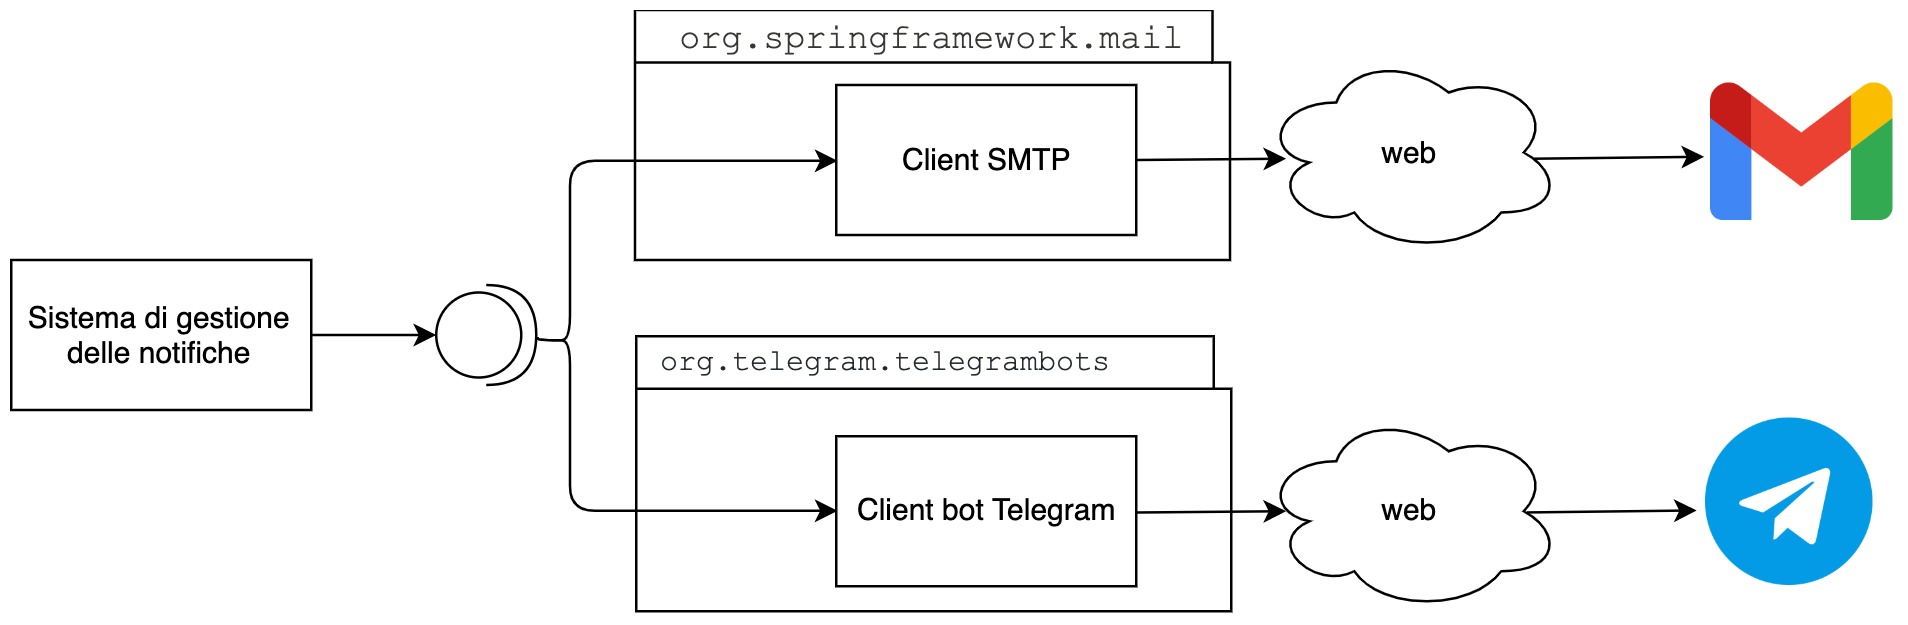
\includegraphics[keepaspectratio = true, width=14cm]{immagini/progettazione/notifica.png}
                            \captionof{figure}{Struttura del sistema di notifica}
                        \end{center}
                        Come si può notare dal diagramma in figura 4.3, fa uso delle seguenti dipendenze:
                        \begin{itemize}
                            \item \texttt{org.springframework.boot:spring-boot-starter-mail} per andare a interfacciarsi con Gmail per la notifica tramite mail;
                            \item \texttt{org.telegram:telegrambots} per andare a interfacciarsi con Telegram per la notifica tramite messaggio su gruppo.
                        \end{itemize} 
            \end{quote}
        \subsubsection{Sistema di pubblicazione}
            Questo sistema, avente come responsabilità la pubblicazione di analisi statistiche sui dati, ha fatto uso del \texttt{MVC design pattern} per il suo sviluppo, così da disaccoppiare la logica tra modello, controller e viste, in modo da rendere modulare il sistema e permettere una potenziale futura migrazione a tipi di viste diverse (per esempio tramite XML) o l'aggiunta di nuovi endpoint.\\
            \begin{quote}
            	\mbox{}%
            	\vspace{-1cm}
                    \subparagraph{Dipendenze esterne}
                    \mbox{} \\
                        Questo sistema è stato, come precedentemente dichiarato, sviluppato seguendo il design pattern MVC, questo appoggiandosi al framework Java, Spring Boot. \\
                        Per questo motivo viene identificato \texttt{org.springframework.boot} come dipendenza esterna. 
            \end{quote}
        \newpage
    \subsection{Logica dell'engine}
        La logica che usa l'engine per raggiungere i suoi obbiettivi può essere riassunta con il diagramma UML riportato in figura 4.4
        \begin{center}
            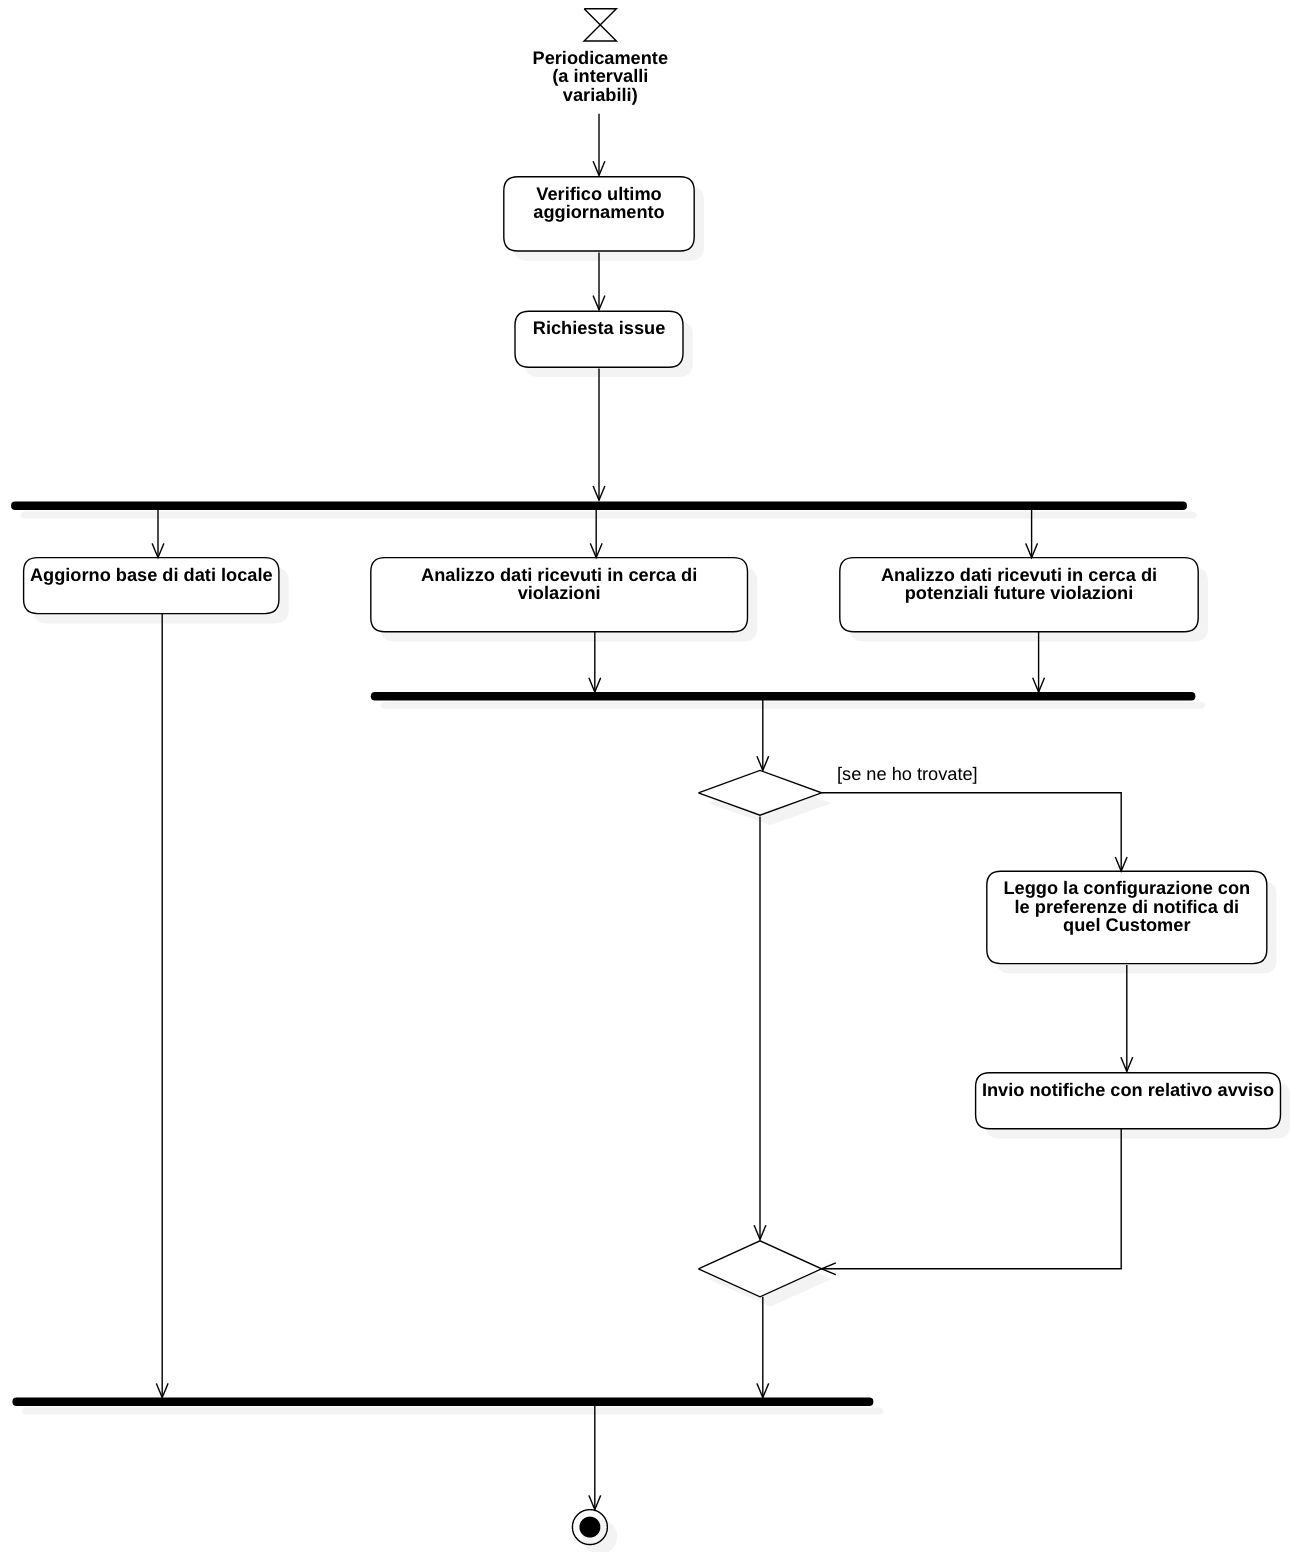
\includegraphics[keepaspectratio = true, width=15cm]{immagini/progettazione/activity.png}
            \captionof{figure}{Diagramma di attività dell'algoritmo dell'engine}
        \end{center}
    
        
\section{Base di dati}
    Il progetto prevede l'uso di una base di dati per il mantenimento locale delle informazioni ottenute dal servizio esterno per la gestione di progetto. \\
    In particolare, questa base di dati ha l'obiettivo di mantenere le informazioni esposte dall'API successivamente descritta. \\
    \par La base di dati prevista è rappresentata dallo schema riportato in figura \S 4.5
    \begin{center}
        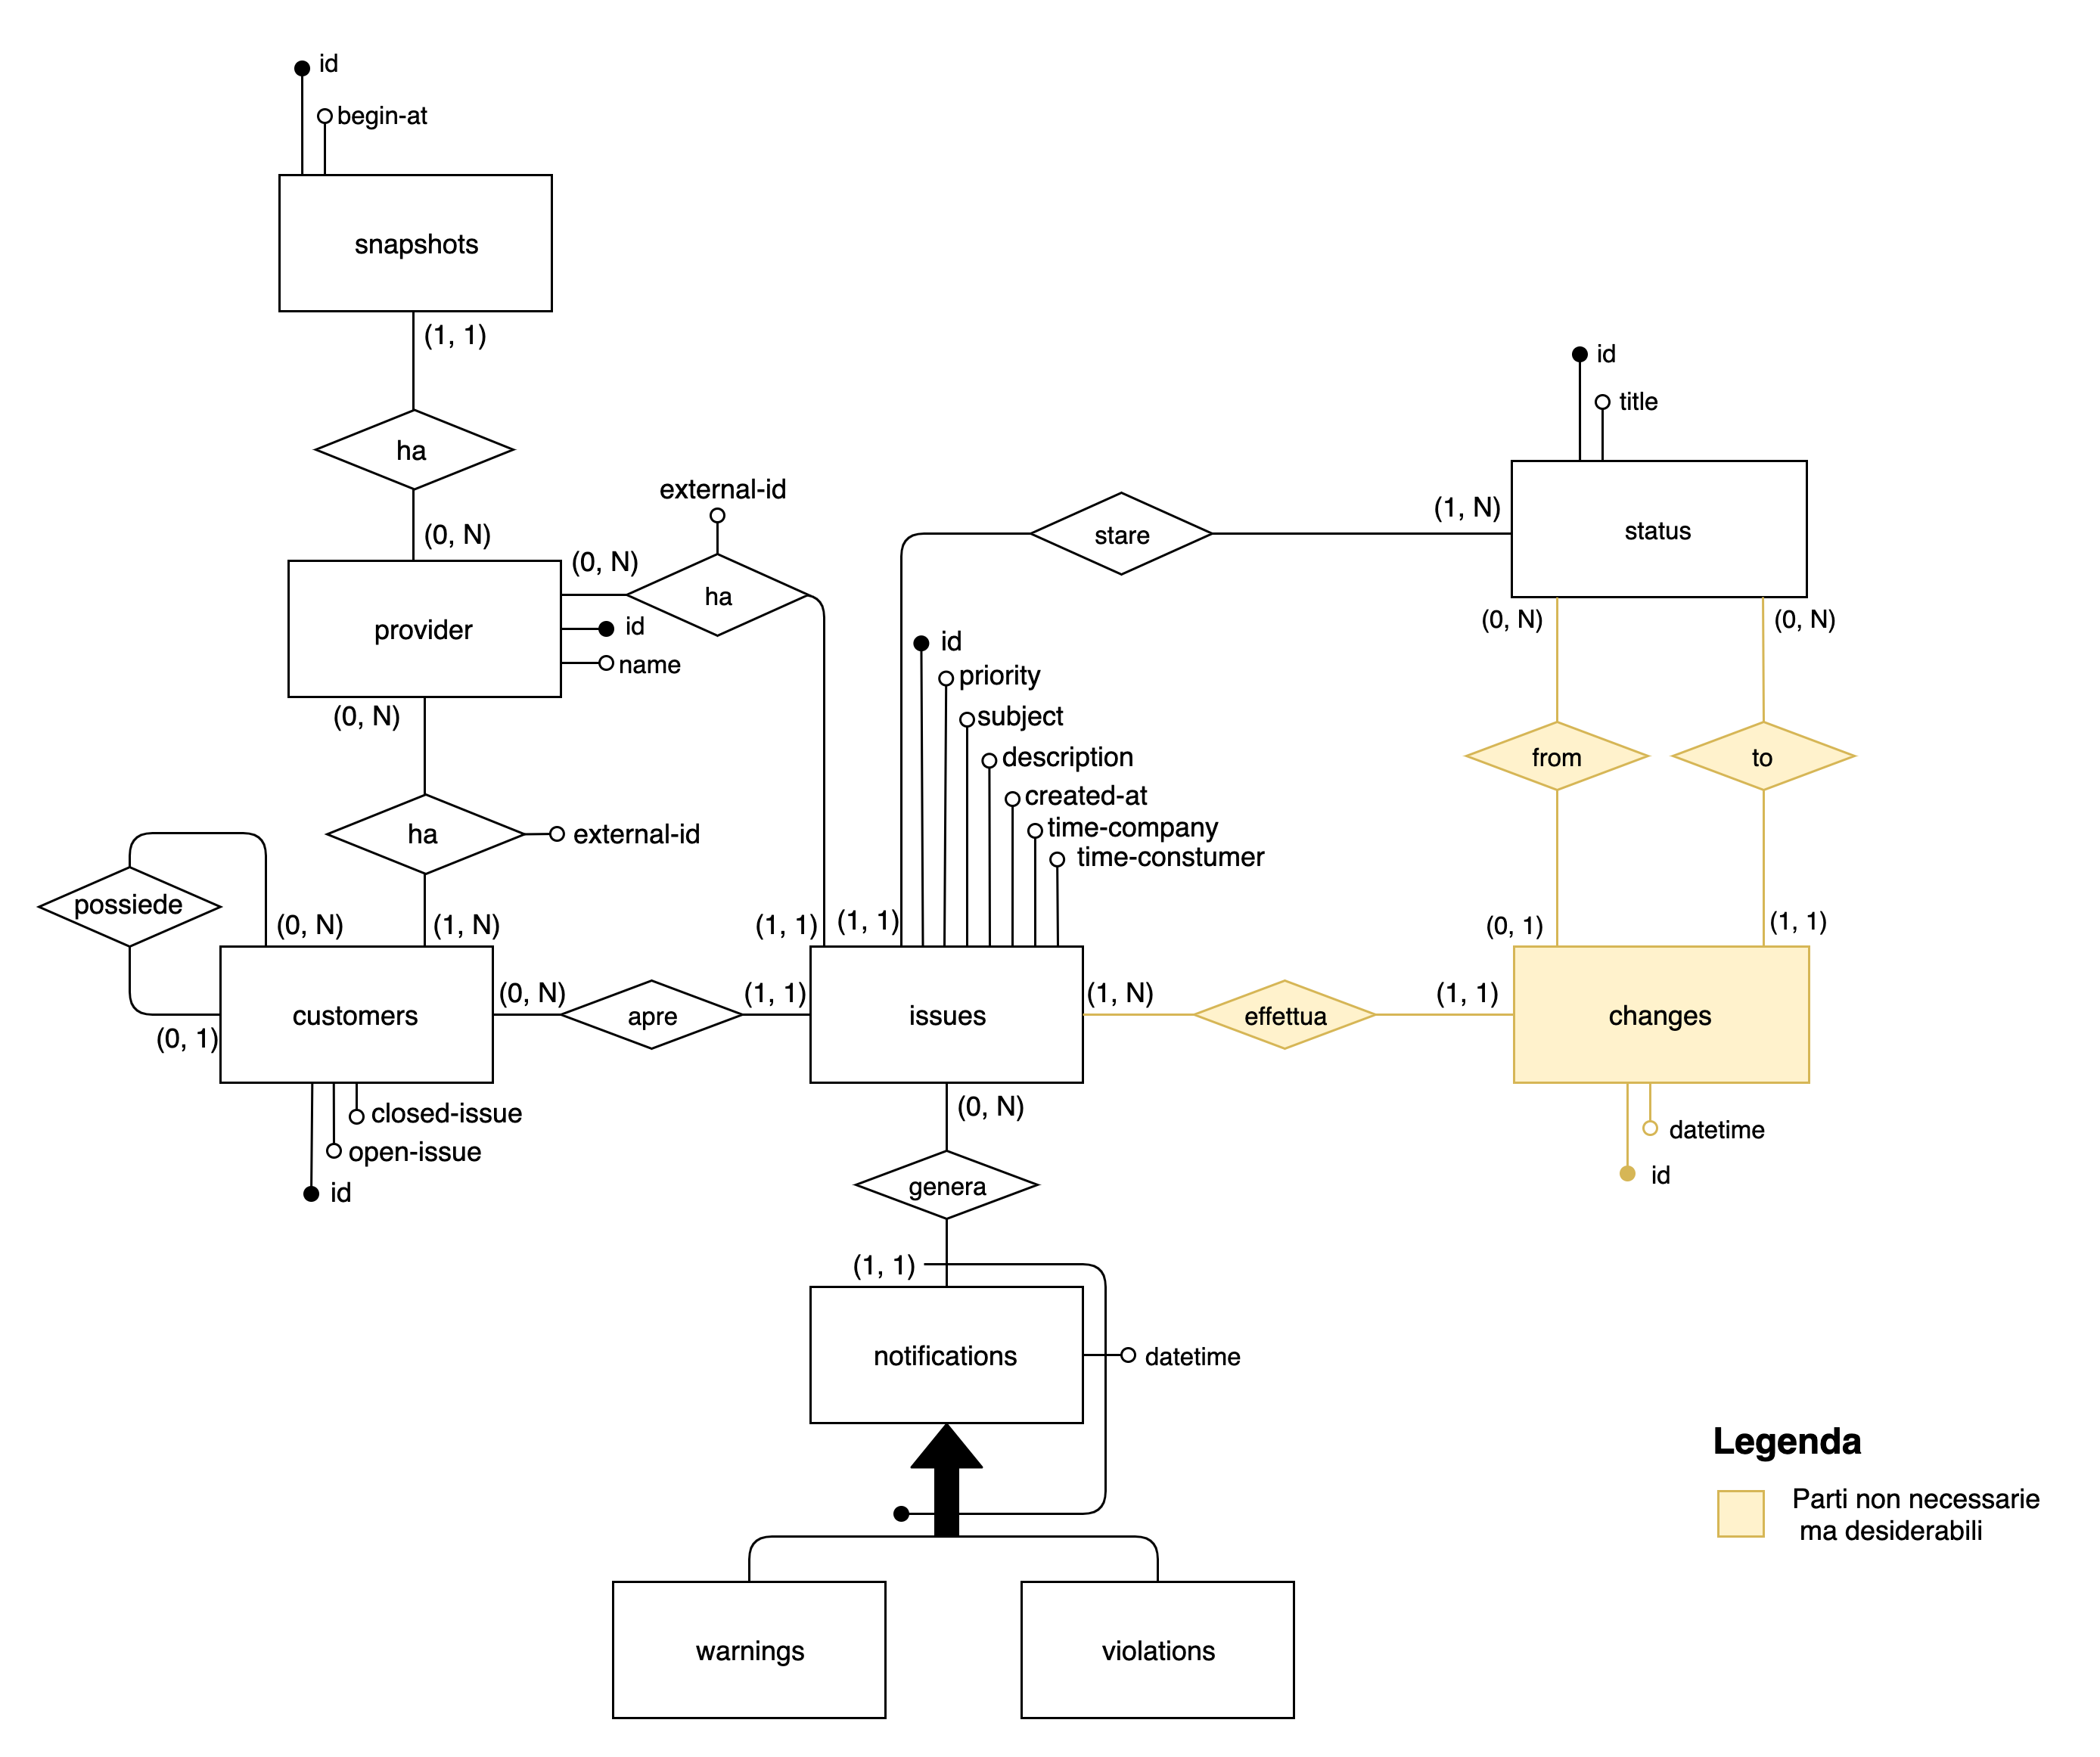
\includegraphics[keepaspectratio = true, width=15cm]{immagini/progettazione/db.png}
        \captionof{figure}{Struttura della base di dati prevista}
    \end{center}
	Nella base di dati son presenti le seguenti entità:
	\begin{itemize}
		\item \texttt{provider}: rappresenta un generico provider dal quale si ottengono dati (inizialmente conterrà solo Redmine);
		\item \texttt{snapshot}: rappresenta un aggiornamento effettuato dal sistema di ottenimento ed è associato al provider per nel quale si ha fatto l'aggiornamento;
		\item \texttt{customer}: rappresenta un qualsiasi customer tracciato dall'engine, i quali son associati a N provider, in modo da poter rappresentare lo stesso customer su più provider esterni;
		\item \texttt{issue}: rappresenta un qualsiasi ticket aperto da un customer su uno dei provider tracciati; esso quindi ha un riferimento al customer che l'ha aperto e al provider nel quale è stato creato;
		\item \texttt{notification}: rappresenta una qualsiasi notifica inviata dall'engine, che può essere di due tipi, \texttt{warning} e \texttt{violation}; tale notifica ha un riferimento all'issue associata;
		\item \texttt{change}: rappresenta una qualsiasi cambio di stato di una issue nel suo ciclo di vita; esso ha un riferimento al suo stato precedente, e al suo nuovo stato;
		\item \texttt{status}: rappresenta un qualsiasi stato che un issue può assumere durante il suo ciclo di vita.
	\end{itemize}
	
    \subsection{Analisi ridondanze}
        Lo schema ER visibile alla sezione precedente, presenta non minimalità, quali:
        \begin{itemize}
            \item \texttt{status} in \texttt{issues}, che potrebbe essere recuperato dallo stato del suo ultimo cambiamento;
            \item \texttt{time-company} e \texttt{time-customer} in \texttt{issues} che potrebbero essere ricalcolate considerando tutti le sue \texttt{changes};
            \item \texttt{open-issue} e \texttt{closed-issue} in \texttt{customers} che potrebbero essere ottenute contando le \texttt{issues} associate.
        \end{itemize} 
        Si è deciso di mantenere queste non-minimalità in modo da ottimizzare la pubblicazione di suddetti dati dall'API, in quanto focus primario del progetto.
    








\section{Endpoint API}
    \subsection{/customer/\{customer-id\}}
        \begin{itemize}
            \item \textbf{Tipo del metodo}: GET;
            \item \textbf{Descrizione}: endpoint per l'ottenimento delle informazioni rispetto a un customer.
            \item \textbf{Parametri}: \\
            \begin{center}
                \rowcolors{2}{lightest-grayest}{white}
                \begin{longtable}{|p{4cm}|p{4cm}|p{6cm}|}
                    \hline
                    \rowcolor{lighter-grayer}
                    \textbf{Nome} & \textbf{Tipo} & \textbf{Descrizione} \\ \hline
                    \texttt{min} & Timestamp GMT+2 & Data minima dell'apertura di ticket da considerare \\ \hline
                    \texttt{max} & Timestamp GMT+2 & Data massima dell'apertura di ticket da considerare \\ \hline
                \end{longtable}
            \end{center}
            \item \textbf{Risposte}: 
            \begin{center}
                \rowcolors{2}{lightest-grayest}{white}
                \begin{longtable}{|p{2.5cm}|p{5.5cm}|p{6cm}|}
                    \hline
                    \rowcolor{lighter-grayer}
                    \textbf{Identificativo} & \textbf{Schema \gloxy{JSON}} & \textbf{Descrizione} \\
                    \hline
                    \endfirsthead
                    200 & 
                    \texttt{
                        \{ \newline 
                            "id": int \newline 
                            "name": string \newline 
                            "issues": int \newline 
                            "violations": int \newline 
                            "avg-pending": float \newline 
                            "avg-resolved": float \newline 
                        \}
                    } 
                    & Risposta contenente:
                    \begin{itemize}
                        \item nome del customer
                        \item numero di issue aperte
                        \item numero di violazioni subite
                        \item tempo medio di presa in carico
                        \item tempo medio di risoluzione
                    \end{itemize}
                    \\ \hline
                    400 & \texttt{\{ \newline "message": string \newline \}} & I timestamp forniti non sono validi
                    \\ \hline
                    404 & \texttt{\{ \newline "message": string \newline \}} & L'id del customer fornito non è stato trovato
                    \\ \hline
                \end{longtable}
            \end{center}
            \item \textbf{HTTP headers}: 
            \begin{itemize}
                \item \textbf{Content-Type:} \texttt{application/json} ;
            \end{itemize}
        \end{itemize}
    
    
    \newpage
    \subsection{/issue/\{issue-id\}}
        \begin{itemize}
            \item \textbf{Tipo del metodo}: GET;
            \item \textbf{Descrizione}: endpoint per l'ottenimento delle informazioni rispetto a un issue.
            \item \textbf{Parametri}: \\
            Nessuno
            \item \textbf{Risposte}: 
            \begin{center}
                \rowcolors{2}{lightest-grayest}{white}
                \begin{longtable}{|p{2.5cm}|p{5.5cm}|p{6cm}|}
                    \hline
                    \rowcolor{lighter-grayer}
                    \textbf{Identificativo} & \textbf{Schema \gloxy{JSON}} & \textbf{Descrizione} \\
                    \hline
                    \endfirsthead
                    200 & 
                    \texttt{
                        \{ \newline 
                        "id": int \newline 
                        "customer": int \newline 
                        "status": string \newline 
                        "priority": string \newline 
                        "subject": string \newline 
                        "description": string \newline 
                        "start-date": string(yyyy-mm-gg) \newline 
                        "time-company": int \newline 
                        "time-client": int \newline 
                        \}
                    } 
                    & Risposta contenente :
                    \begin{itemize}
                        \item id dell'issue
                        \item nome del customer
                        \item stato dell'issue
                        \item priorità dell'issue
                        \item oggetto dell'issue
                        \item descrizione dell'issue
                        \item data di apertura dell'issue
                        \item tempo che è stato in carico a Euronovate
                        \item tempo che è stato in carico al Customer
                    \end{itemize}
                    \\ \hline
                    404 & \texttt{\{ \newline "message": string \newline \}} & L'id dell'issue fornito non è stato trovato
                    \\ \hline
                \end{longtable}
            \end{center}
            \item \textbf{HTTP headers}: 
            \begin{itemize}
                \item \textbf{Content-Type:} \texttt{application/json} ;
            \end{itemize}
        \end{itemize}
    
    
    
    
    \newpage
    \subsection{/issues}
        \begin{itemize}
            \item \textbf{Tipo del metodo}: GET;
            \item \textbf{Descrizione}: endpoint per ottenere informazioni statistiche sull'andamento nel tempo delle issue.
            \item \textbf{Parametri}: \\
                \begin{center}
                    \rowcolors{2}{lightest-grayest}{white}
                    \begin{longtable}{|p{4cm}|p{4cm}|p{6cm}|}
                        \hline
                        \rowcolor{lighter-grayer}
                        \textbf{Nome} & \textbf{Tipo} & \textbf{Descrizione} \\ \hline
                        \texttt{min} & Timestamp GMT+2 & Data minima dell'apertura di ticket da considerare \\ \hline
                        \texttt{max} & Timestamp GMT+2 & Data massima dell'apertura di ticket da considerare \\ \hline
                        \texttt{group-by} & string & String rappresentante la politica di raggruppamento; deve essere una tra:
                        \begin{itemize}
                            \item day
                            \item month (default)
                            \item year
                        \end{itemize}
                            \\ \hline
                    \end{longtable}
                \end{center}
            \item \textbf{Risposte}: 
            \begin{center}
                \rowcolors{2}{lightest-grayest}{white}
                \begin{longtable}{|p{2.5cm}|p{5.5cm}|p{6cm}|}
                    \hline
                    \rowcolor{lighter-grayer}
                    \textbf{Identificativo} & \textbf{Schema \gloxy{JSON}} & \textbf{Descrizione} \\
                    \hline
                    \endfirsthead
                    200 & 
                    \texttt{
                        [
                        \{ \newline 
                        "begin-date": string (yyyy-mm-gg) \newline 
                        "created-issues": int \newline 
                        "open-issues": int \newline 
                        "violations": int \newline 
                        \},\newline 
                        ...\newline 
                        ]
                    } 
                    & Risposta contenente una collezione di oggetti contenenti:
                    \begin{itemize}
                        \item la data di inizio periodo
                        \item numero di issue aperte in quel periodo
                        \item numero di issue aperte all'inizio di quel periodo 
                        \item numero di violazioni notificate in quel periodo
                    \end{itemize}
                    \\ \hline
                    400 & \texttt{\{ \newline "message": string \newline \}} & I timestamp forniti non sono validi o il campo di raggruppamento non contiene uno dei valori definiti.
                    \\ \hline
                \end{longtable}
            \end{center}
            \item \textbf{HTTP headers}: 
            \begin{itemize}
                \item \textbf{Content-Type:} \texttt{application/json} ;
            \end{itemize}
        \end{itemize}
    \newpage
    
    
    
\section{Tecnologie e strumenti}
    Durante la fase di sviluppo son stati necessari strumenti per la verifica e lo sviluppo dei vari componenti, quali:
    \begin{itemize}
    	\item \texttt{Java}[1] : linguaggio di programmazione con il quale si è sviluppato il progetto per la maggior parte, principalmente la sua versione 11 LTS; \\
    	Esso ha permesso una facile esportazione del progetto in macchine diverse in quanto platform-indipendent grazie alla JVM; \\
    	Grazie al suo approccio ad oggetti alla programmazione, ha permesso una alta modularità del sistema, permettendo di isolare i sistemi tra di loro;
    	\item \texttt{JSON} : markup usato per la pubblicazione dei dati dell'API, scelto rispetto a XML per la sua minore verbosità e per la sua facile integrazione con client esterni;
    	\item \texttt{XML} : markup usato per il salvataggio dei dati sui customers, sui canali di notifica e sugli orari di lavoro su disco. \\
    	Grazie alla sua nativa integrazione con Spring, non c'è stata la necessità di librerie esterne per la sua deserializzazione;
    	\item \texttt{Git} : sistema di versionamento usato per il tracciamento del progetto;
    	\item \texttt{CodeCommit} : servizio di hosting online per repository che supporta Git, di proprietà AWS;
    	\item \texttt{Spring Boot} : framework principale del progetto a base Java, estremamente diffuso in ambito aziendale/lavorativo. \\
    	Esso ha permesso l'utilizzo di dependency injection in tutto il progetto, così da sollevare le varie classi della creazione degli oggetti. Ha permesso inoltre un'implementazione del sistema di pubblicazione usando  il pattern MVC, separando modello, vista e logica di ottenimento dati;
    	\item \texttt{Redmine SDK}[3] : libreria usata per interfacciarsi con le API di Redmine, open-source, presente su Github, così da potersi sollevare dall'onere di sviluppare la logica di ottenimento dei dati dal provider esterno;
    	\item \texttt{Telegram SDK}[5] : libreria usata per interfacciarsi con le API di Telegram, open-source, presente in Github, così da non dover sviluppare la logica di comunicazione con Telegram;
    	\item \texttt{Spring Mail}[6] : libreria usata per interfacciarsi con server mail, la quale supporta la connessione a qualsiasi client SMTP, trai quali Gmail, servizio scelto per il progetto;
    	 \item \texttt{IntelliJ IDEA} : IDE usato per lo sviluppo del progetto;
    	\item \texttt{JUnit} : libreria Java per lo sviluppo di test di unità, usato per lo sviluppo di una suite di test della parte algoritmica del progetto;
    	\item \texttt{Postman} : applicazione per interrogazione e testing di API;
    	\item \texttt{Docker} : prodotto usato per il deploy finale del prodotto;
    	\item \texttt{SQL} : linguaggio per database basati sul modello relazionale, usato per il mantenimento dei dati, in particolare usato con DMBS  \texttt{PostgreSQL};
    	\item \texttt{pgAdmin} : client per la gestione di DBMS \texttt{PostgreSQL}.
    \end{itemize}
    
    
    
    
    
    
\section{Sviluppo}
	In questa sezione verranno trattate la parti principali e più interessanti della codifica e realizzazione del progetto.
	
	\subsection{Ordine di sviluppo}
		Come descritto in precedenza, il prodotto prevede dei sistemi isolati tra di loro, ognuno con il proprio obiettivo. \\
		Appunto per la loro peculiarità di essere isolati, si è proceduto allo sviluppo di ognuno di essi in modo sequenziale, passando al successivo solo quando quello corrente è completo e funzionante. \\
		In particolare, lo sviluppo ha seguito il seguente ordine:
		\begin{enumerate}
			\item Base di dati;
			\item Layer di persistenza;
			\item Sistema di ottenimento;
			\item Sistema di aggiornamento;
			\item Sistema di analisi;
			\item Sistema di notifica;
			\item Sistema di pubblicazione.
		\end{enumerate}
		Successivo allo sviluppo di ognuno di questi punti, si è svolto un allineamento con il tutor aziendale, per assicurarsi che il sistema prodotto fosse completo e funzionale.\\
		Seguendo questo ordine è stato più facile sviluppare i sistemi il più isolati possibili, e quindi concentrandosi sugli obiettivi di essi e il come potessero essere usati, ma non come sarebbero stati usati. \\
	\subsection{Differenze dalla progettazione}
		Per quanto il prodotto sviluppato somigli molto a quello pensato durante la fase di progettazione, son state necessarie alcune modifiche, per correggere alcuni aspetti non previsti in fasi precedenti, in particolare:
		\begin{itemize}
			\item Sistema di aggiornamento: questo sistema non era previsto dalla progettazione, ma considerata la tarda notifica della granularità dei vincoli presenti nelle SLA, è stato necessario introdurlo per mantenere consistenti le non minimalità presenti nella base di dati;
			\item Algoritmo calcolo tempo su orario lavorativo: è stato necessario lo sviluppo di alcune classi di supporto per i vari sistemi per la gestione delle tempistiche con ottica lavorativa, quindi considerando un orario lavorativo;
			\item Algoritmo di invio di notifiche estendibile per le varie necessità dei canali, per evitare di andare a violare definiti dai rate limiter dei vari sistemi esterni;
			\item sviluppo di un orchestratore per i vari manager dei vari sistemi (Engine).
		\end{itemize}
		Questi nuovi componenti non hanno però portato un ritardo allo sviluppo in quanto fondamentali ma relativamente semplici da implementare. \\
		Considerate queste modifiche, il progetto finale ha un'architettura che può essere descritta dallo schema riportato in figura 4.6
		\begin{center}
			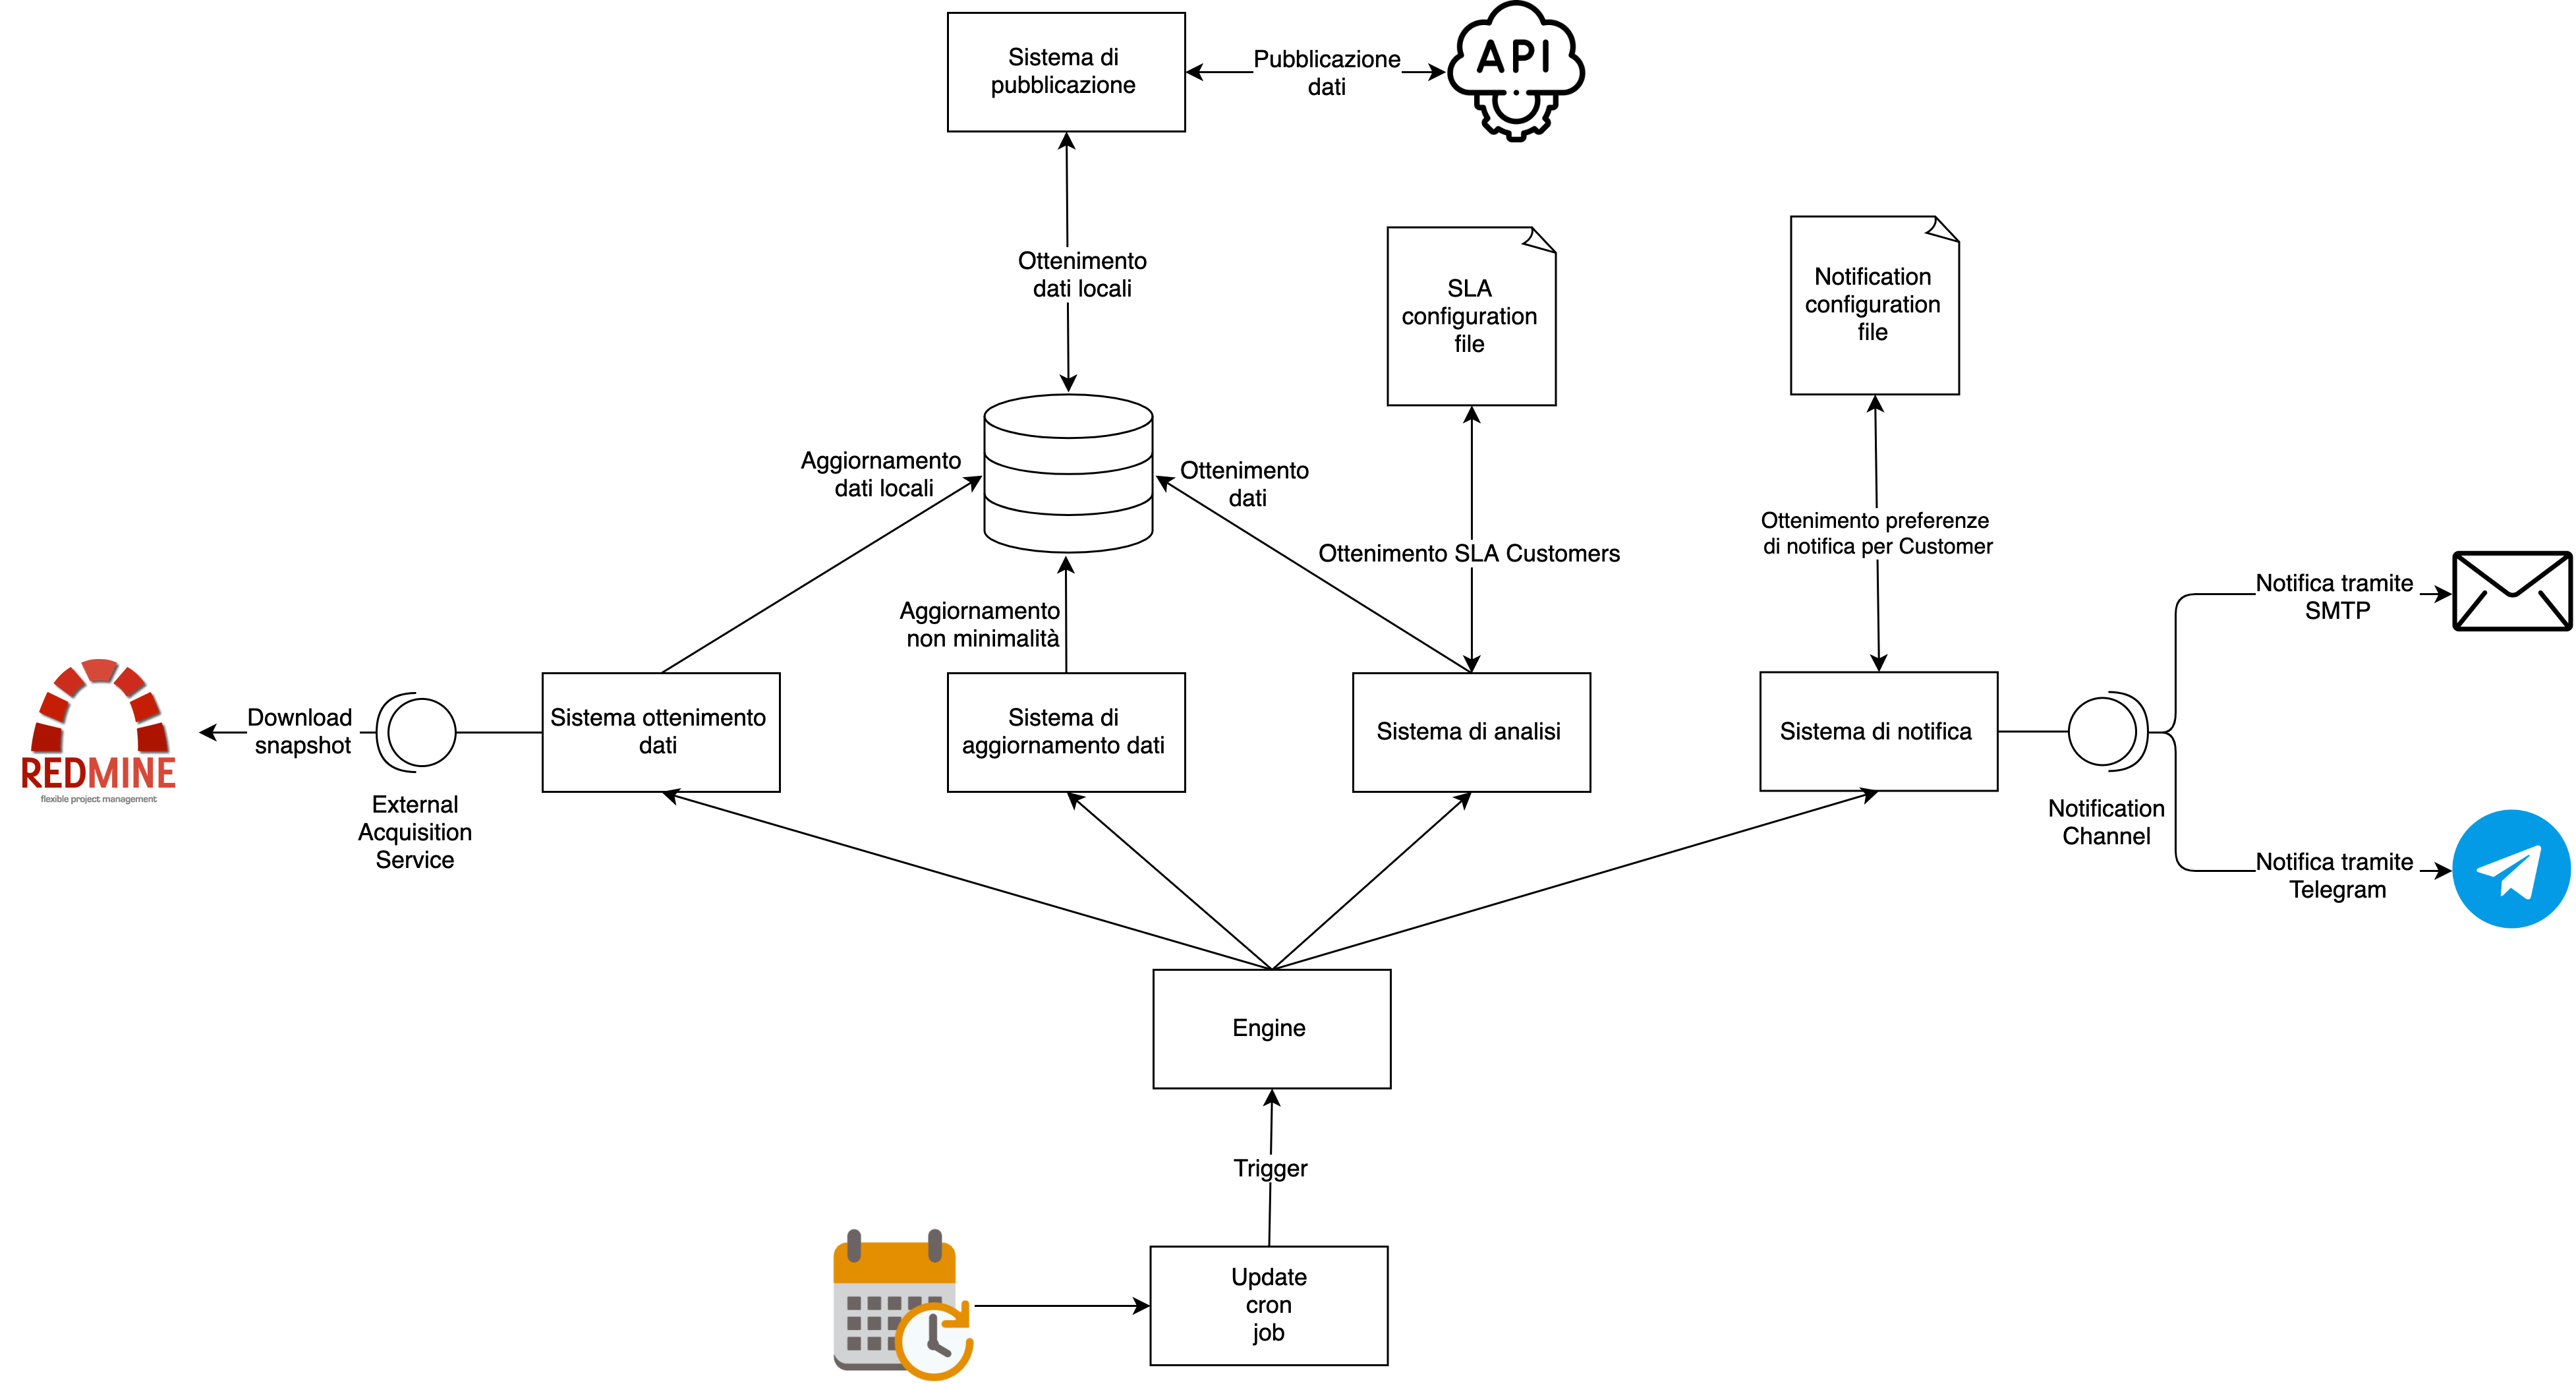
\includegraphics[keepaspectratio = true, width=16cm]{immagini/architettura-finale.png}
			\captionof{figure}{Architettura finale del progetto}
		\end{center}
		
	\subsection{Particolarità }
		Il prodotto è stato sviluppato con alcune caratteristiche ben definite fin dall'inizio come pilastri principali, quali:
		\begin{itemize}
			\item indipendenza dal provider esterno per l'ottenimento dei dati;
			\item facile estensione dei canali di notifica disponibili;
			\item configurabile tramite file XML.
		\end{itemize}
		\subsubsection{Sistema di ottenimento}
			Il sistema di ottenimento doveva essere sviluppato tenendo a mente che un giorno si potesse migrare a un provider esterno diverso da Redmine, e che tale migrazione dovesse richiedere lo sviluppo del minor codice possibile. \\
			Tale obiettivo si è raggiunto con un esteso utilizzo di 2 design pattern, quali:
			\begin{itemize}
				\item \texttt{Object Adapter};
				\item \texttt{Strategy}.
			\end{itemize}
			Tali design pattern si possono vedere applicati nel diagramma UML riportato in figura 4.7 che descrive l'effettiva implementazione di questo sistema.
   			\begin{center}
				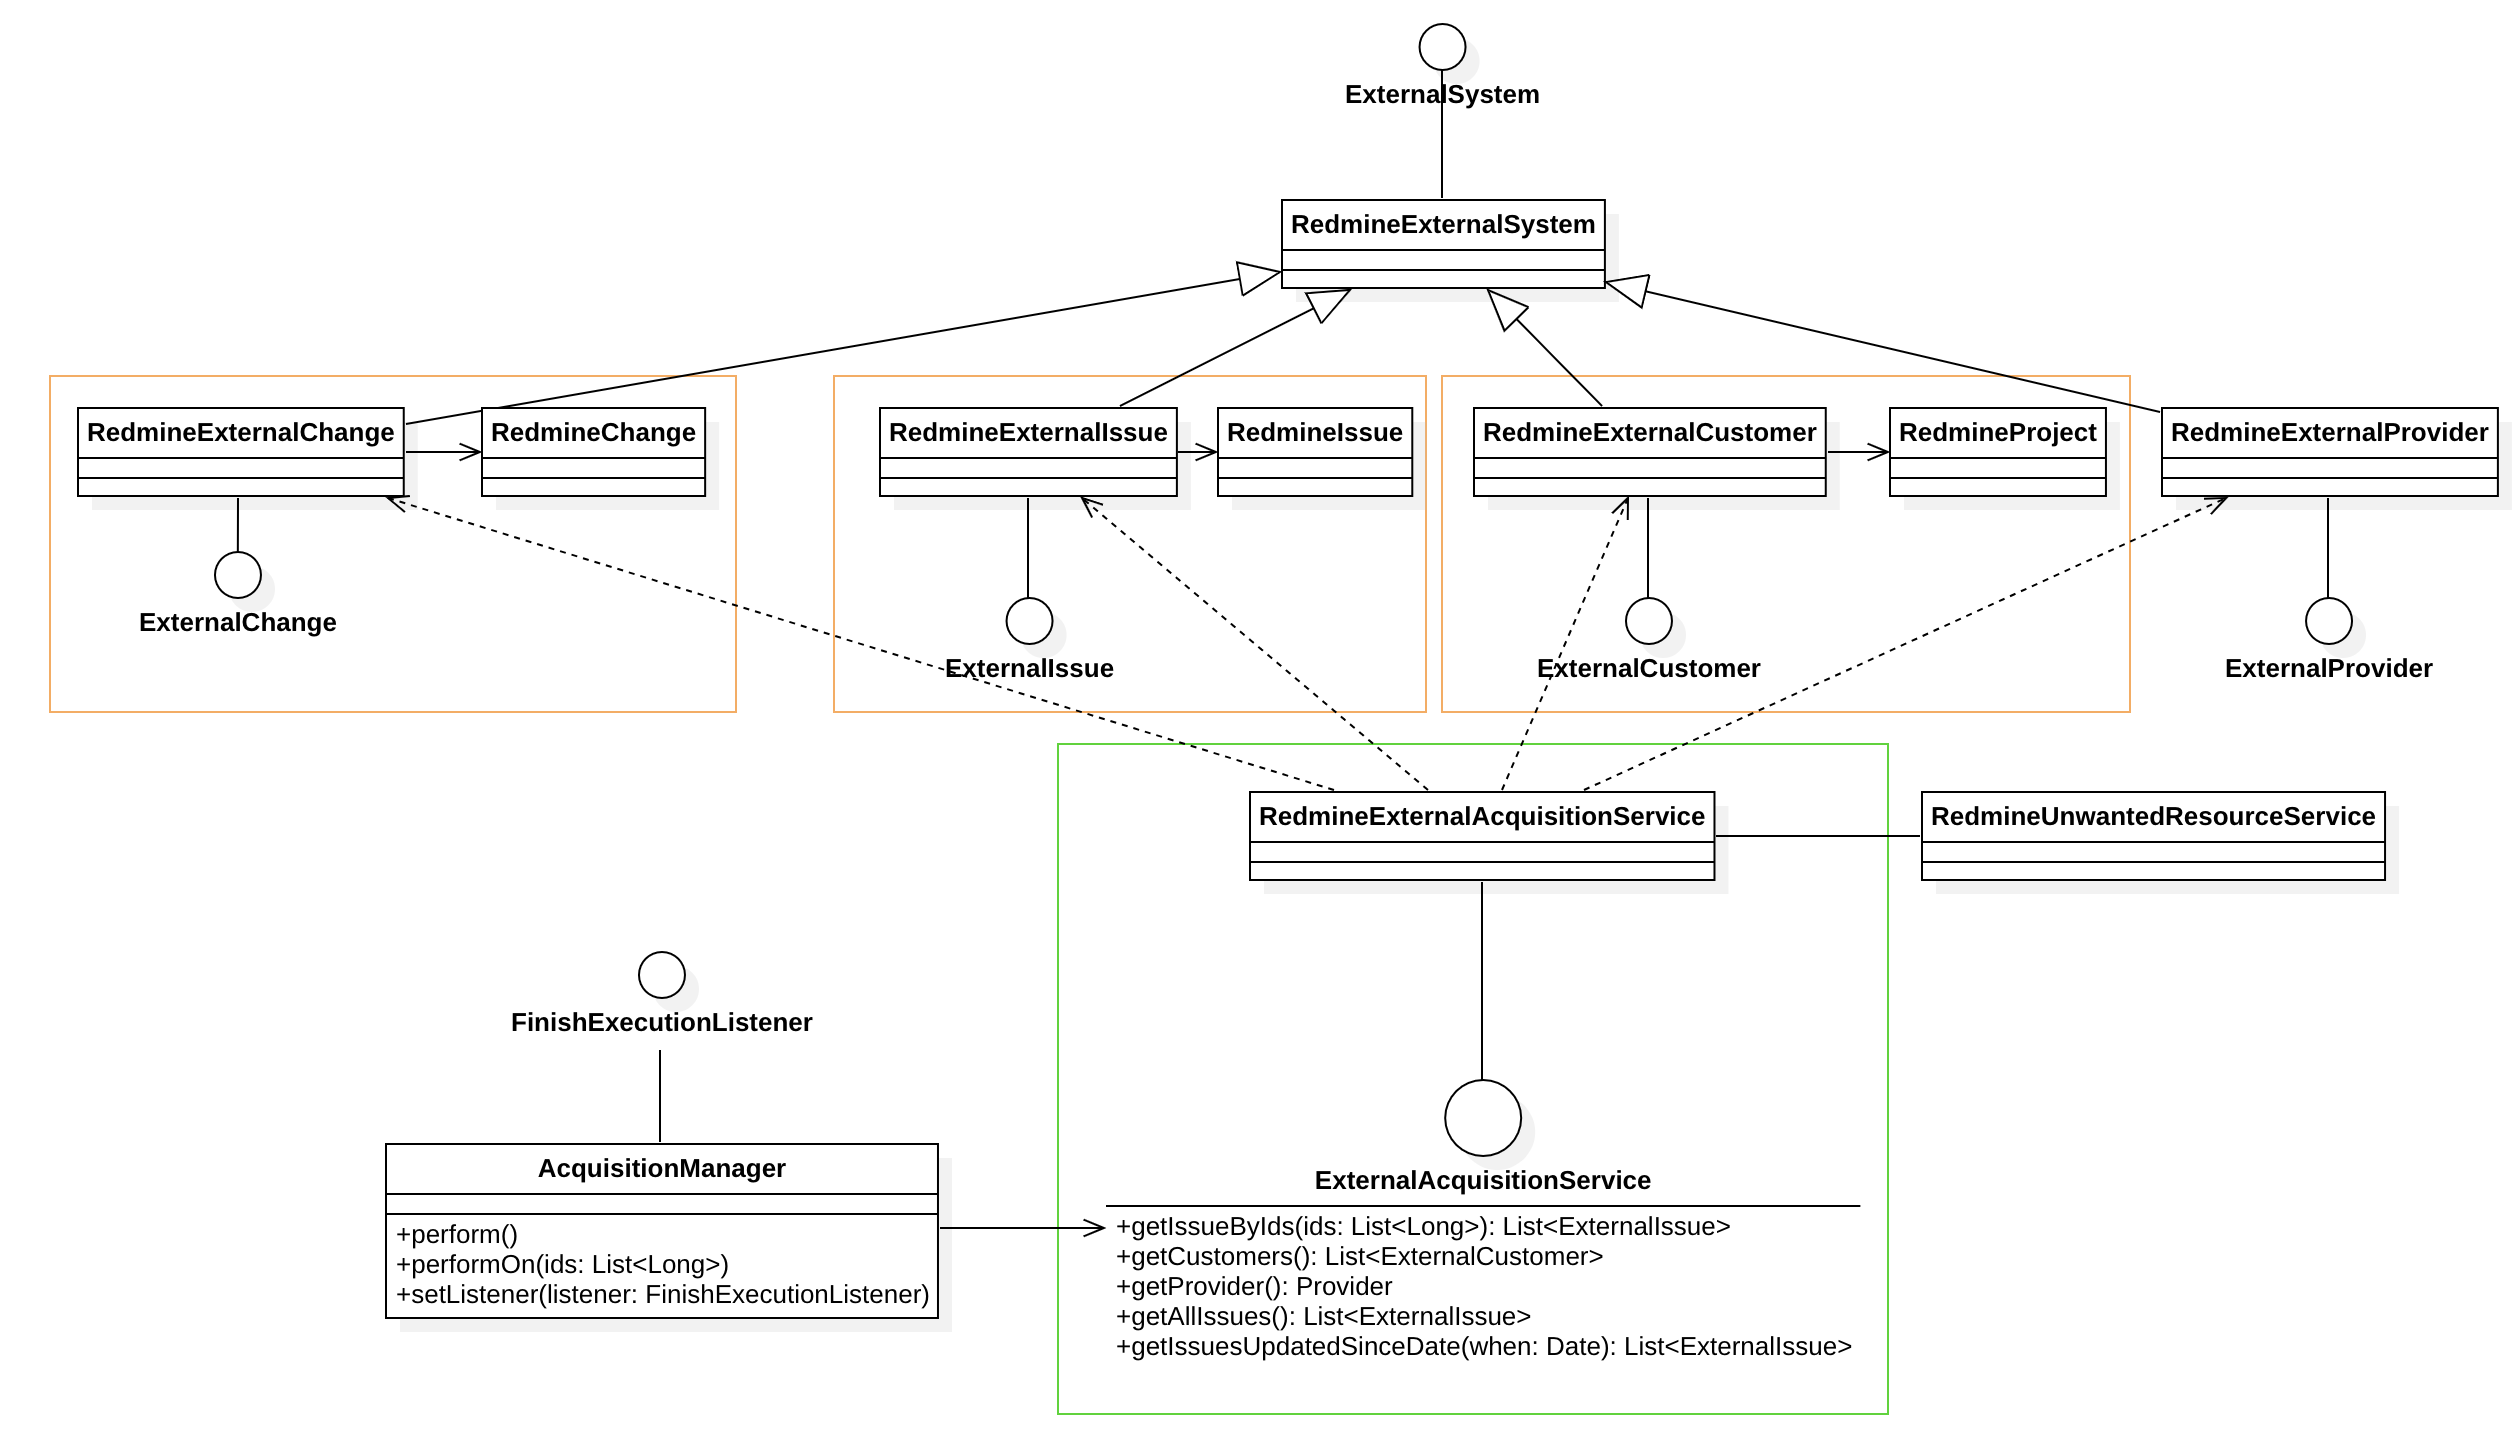
\includegraphics[keepaspectratio = true, width=16cm]{immagini/ottenimento.png}
				\captionof{figure}{UML sistema di ottenimento dati}
			\end{center}
			In arancione si denota l'applicazione del design pattern \texttt{Adapter}, mentre in verde l'applicazione del design pattern \texttt{Strategy}. \\
			Come si può notare, la classe responsabile della logica di ottenimento dei dati,\\ \texttt{AcquisitionManager}, comunica con il sistema esterno di ottenimento dati tramite un'interfaccia; essa definisce i metodi necessari per la \texttt{strategy}, adattando i valori trattati da essa tramite le interfacce usate per l'implementazione del design pattern \texttt{Adapter}. In questo modo si è creata un'indipendenza completa dalla classe responsabile della logica di aggiornamento dei dati \texttt{AcquisitionManager} e la classe responsabile del reperimento dei dati dal provider esterno \texttt{RedmineExternalAcquisitionService}.\\
			Son state quindi poi sviluppate  le classi \texttt{adapter} necessarie per adattare i vari oggetti restituiti dall'SDK di Redmine, a tali interfacce.\\
			In questo modo, se un domani si decidesse di cambiare provider, sarà necessaria l'implementazione della \texttt{strategy} \texttt{ExternalAcquisitionService} e dei relativi \texttt{adapter} per i dati ottenuti, mentre la logica di gestione di tali dati invariata, al mantenimento degli invarianti richiesti dalle interfacce.\\
		\subsubsection{Sistema di notifica}
			Il sistema di notifica doveva essere sviluppato in modo da permettere l'implementazione di nuovi sistemi di notifica.\\
			A tale requisito, si è scoperto in fase di codifica anche la necessità di permettere politiche di invio diverse per ogni canale, in quanto per esempio, Telegram non permette l'invio di più di 20 messaggi al minuto, mentre Gmail permette l'invio di al massimo 60 mail al minuto. \\
			Per far fronte al primo requisito, si è utilizzato il design pattern \texttt{Strategy} per lo sviluppo dei vari canali, mentre per il secondo si è usato il meccanismo del \texttt{Double Dispatch} fornito dal design pattern \texttt{Visitor}.\\
			Tali design pattern possono essere osservati nel  diagramma UML riportato in figura 4.8, che descrive l'effettiva implementazione di questo sistema.
			\begin{center}
				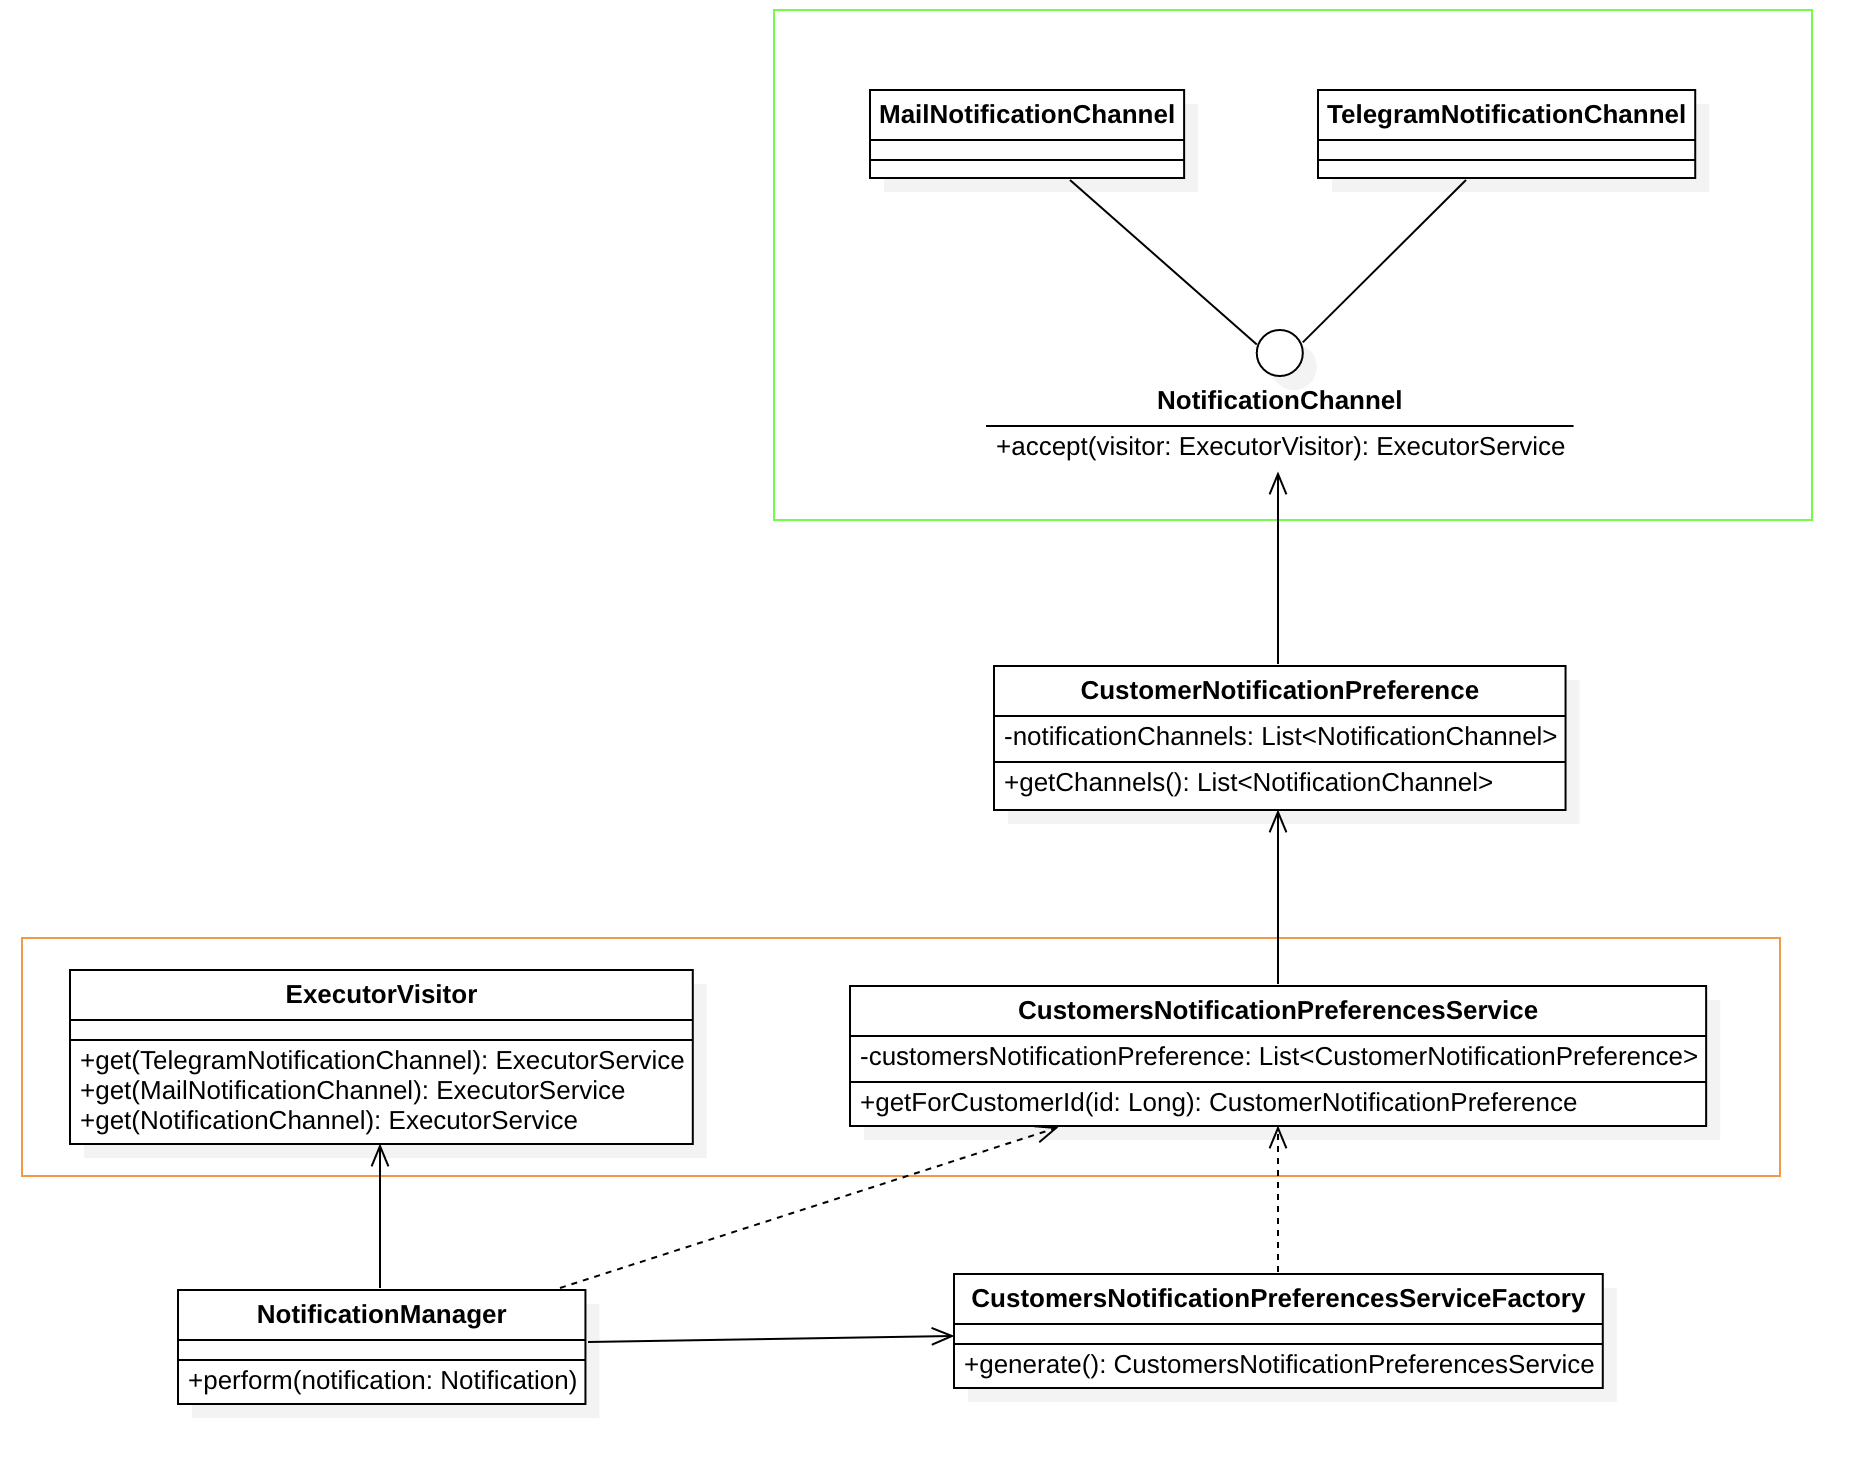
\includegraphics[keepaspectratio = true, width=16cm]{immagini/notifica.png}
				\captionof{figure}{UML sistema di notifica}
			\end{center}
			In giallo si può vedere l'applicazione del design pattern \texttt{Visitor}, che permetterà al sistema di ottenere un \texttt{ExecutorService} dedicato per ogni canale di notifica, e uno di default nel caso fossero presenti canali di notifica senza particolari esigenze di rate limiting. \\
			In particolare, per Telegram ritornerà un \texttt{ExecutorService} con pause di 3 secondi tra ogni \texttt{Runnable} fornitogli,  per Mail ritornerà un \texttt{ExecutorService} con pause di 0.5 secondi tra ogni \texttt{Runnable} fornitogli, mentre per il canale di default ritornerà un \texttt{CachedExecutorService} che permetterà il riutilizzo di \texttt{Thread} già istanziati.\\
			In verde invece si può vedere la \texttt{strategy} applicata ai due canali identificati durante la fase di analisi dei requisiti, la quale permetterà l'estensione a qualsiasi altro canale di notifica, a patto che implementi la sua interfaccia.\\
		\subsubsection{Gestione della configurazione}
			Il progetto richiedeva la possibilità di definire alcuni dati tramite file esterni. \\
			Alcune di queste informazioni sono:
			\begin{itemize}
				\item SLA dei customer (e SLA di default);
				\item orari di lavoro dei customer (e orario di default);
				\item canali di notifica per ogni customer (e canali di default);
				\item orario di lavoro dell'azienda.
			\end{itemize}
			Tali file dovevano essere esterni al progetto così che, una volta creato il \texttt{JAR} e fatto il deploy, fosse possibile modificarli.\\
			Per ottenere ciò, son state create delle \texttt{Factory} per tali oggetti che andranno a deserializzare i file \texttt{XML} richiesti a runtime, con alcune politiche di fallback in caso di errore di lettura. \\
			All'avvio poi, basterà passare come parametro di esecuzione il path al quale sono presenti questi file.\\
		\subsubsection{Engine}
			L'\texttt{Engine}, come si può vedere nel diagramma riportato in figura 4.7, è l'orchestratore dei vari sistemi. \\
			Esso è responsabile dell'esecuzione dei vari manager dei sistemi nell'ordine corretto, e nel caso, della gestione degli errori. \\
			Essendo i vari sistemi stati sviluppati per essere usati ad eventi, l'implementazione di questo servizio non dovrà far altro che collegare i vari listeners dei manager, con i relativi eventi. \\
\iffalse			L'\texttt{Engine} sviluppato, infine, ha una logica di aggiornamento che potrebbe essere riassunta con il seguente schema:
			\begin{center}
				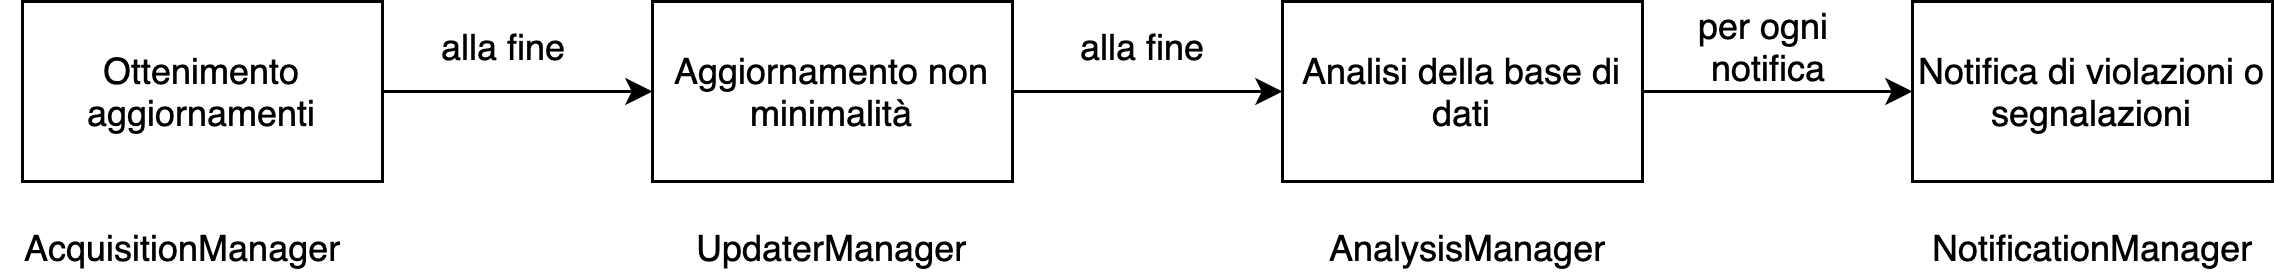
\includegraphics[keepaspectratio = true, width=16cm]{immagini/engine.png}
				\captionof{figure}{Logica di aggiornamento dell'Engine}
			\end{center} \fi
	\subsection{Extra}
		Considerato che lo sviluppo del progetto ha richiesto meno del previsto, si son sviluppe feature aggiuntive esterne al progetto, quali:
		\begin{itemize}
			\item Dashboard Grafana per l'analisi dei dati presenti nella base di dati;
			\item Docker container per il deploy dell'intero progetto, comprendente di engine, dashboard Grafana e database \texttt{PostgreSQL}.
		\end{itemize}
		\subsubsection{Grafana}
			Grafana è uno progetto open-source che mira a semplificare la creazione di dashboard dinamiche per vari tipi di basi di dati. Supporta infatti basi di dati relazionali, a grafo e non relazionali.\\
			Si è proceduto quindi alla creazione di un \texttt{DataSource} per Grafana per la connessione al database usato, e successivamente a una \texttt{Dashboard} connessa a tale \texttt{DataSource} per la visualizzazione di alcuni highlight della base di dati. \\
			Tale dashboard è riportata in figura 4.9
			\newpage
			\begin{center}
				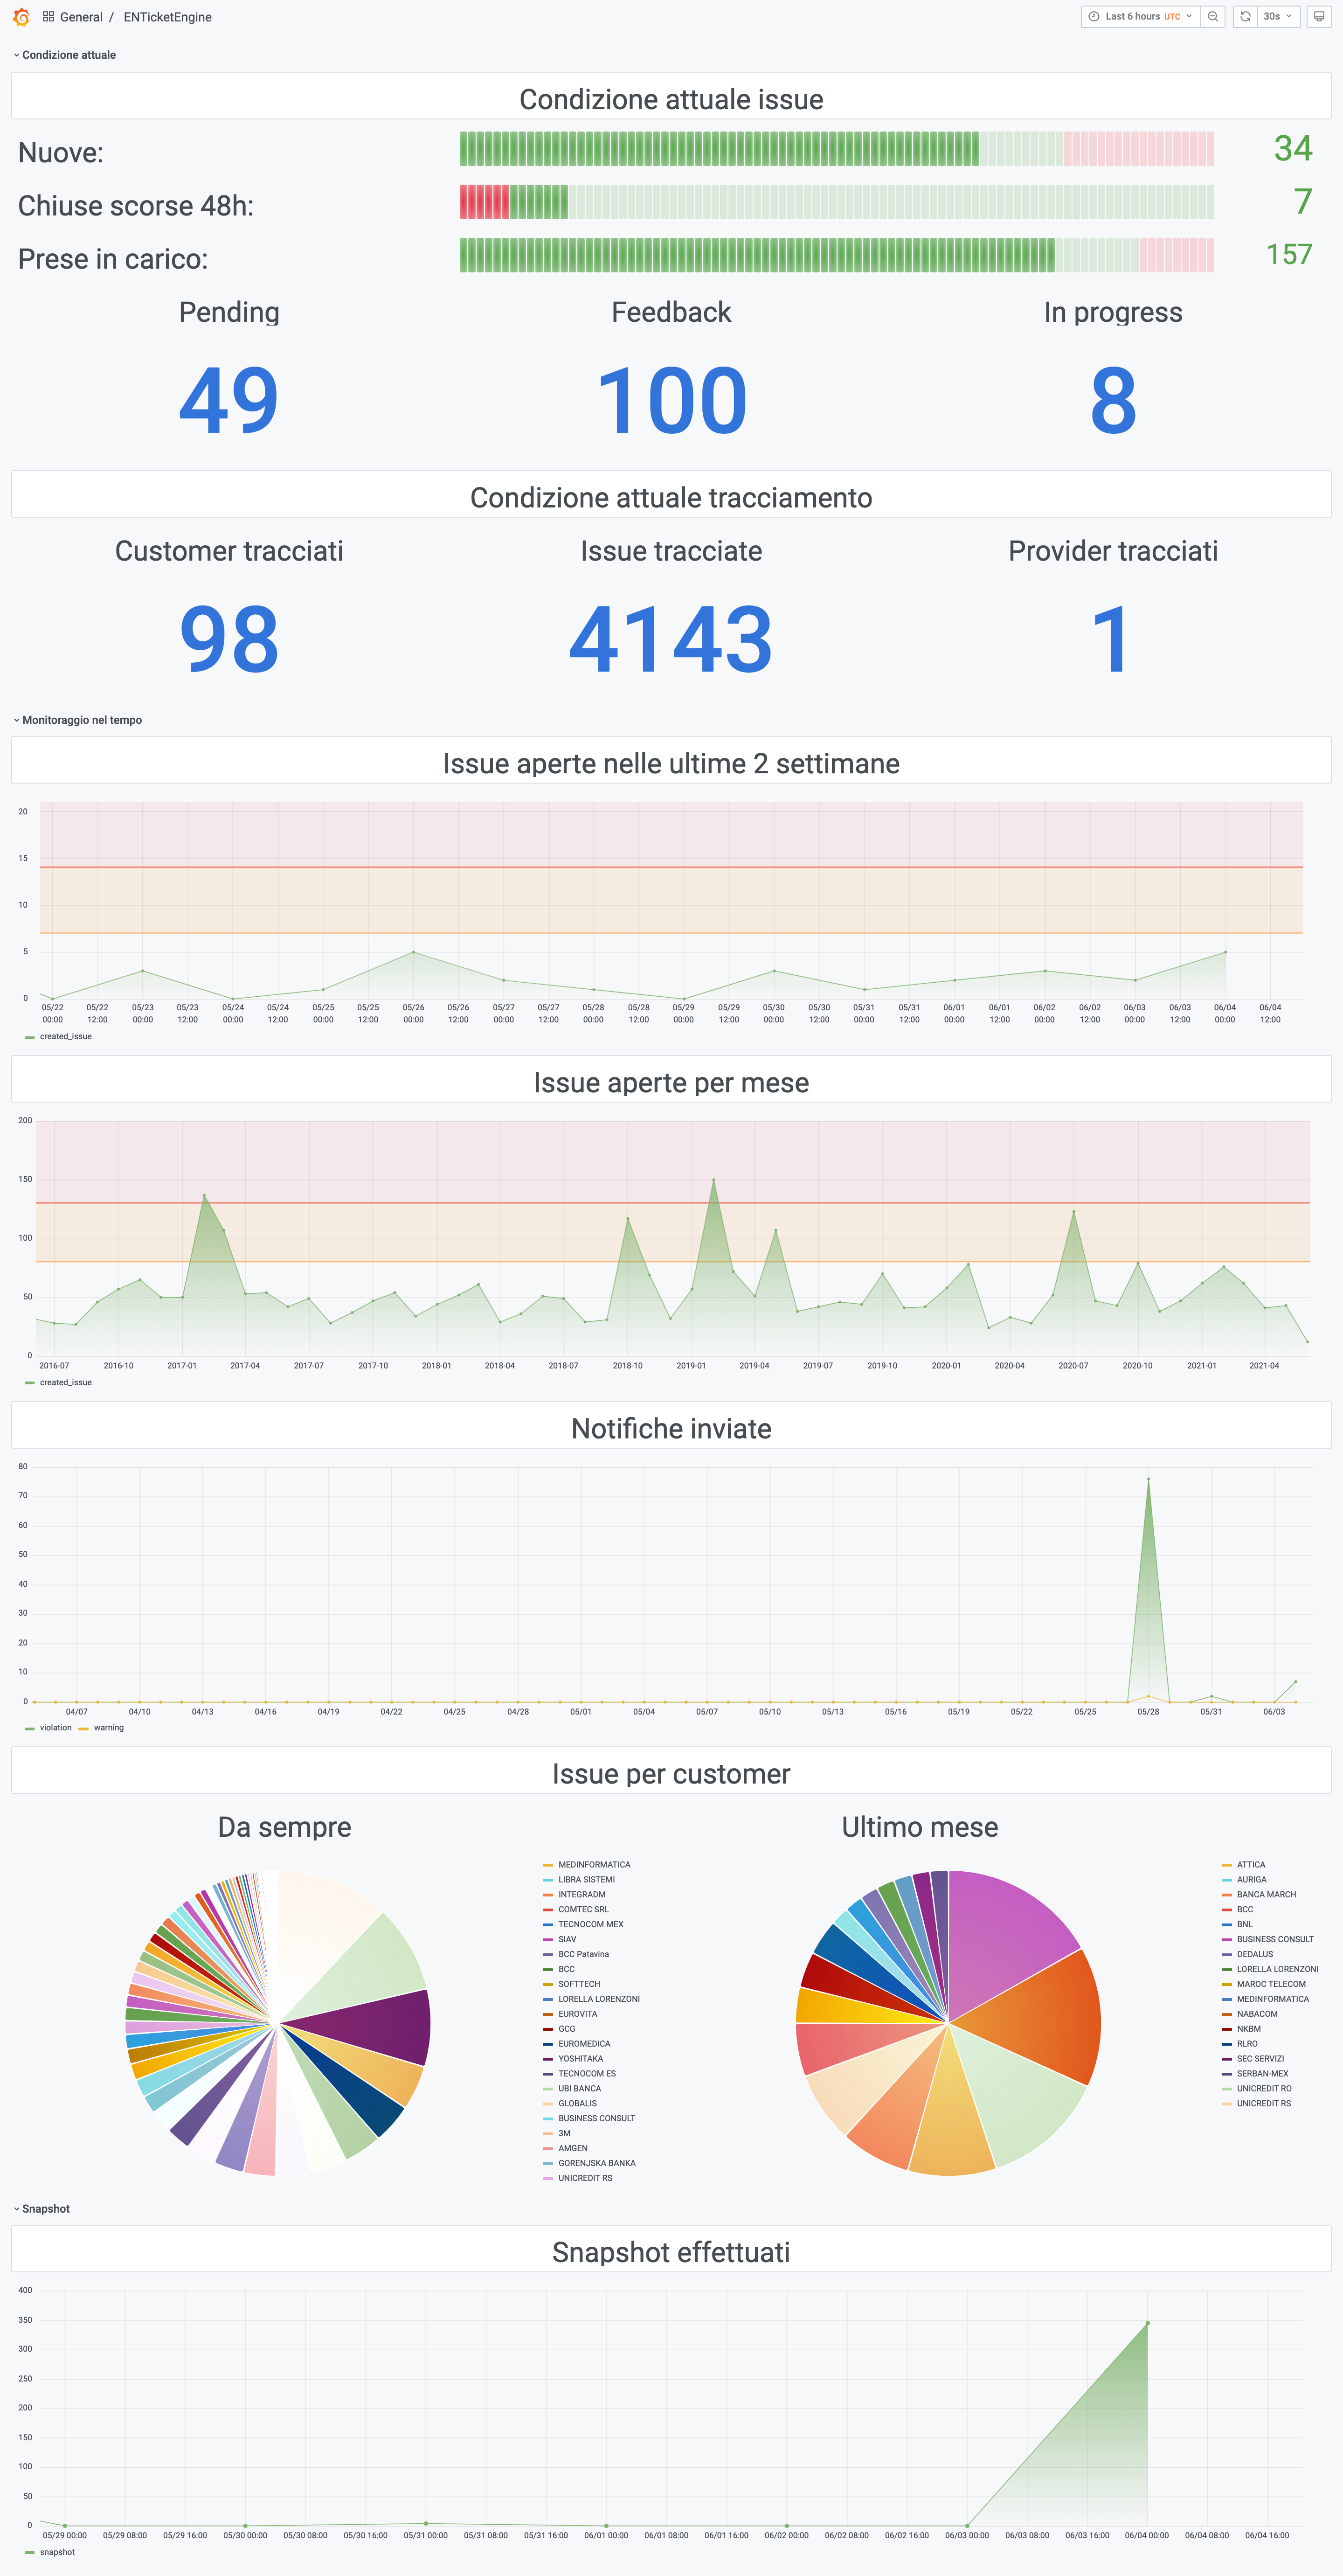
\includegraphics[keepaspectratio = true, height=20cm]{immagini/dashboard.png}
				\captionof{figure}{Dashboard Grafana}
			\end{center}
			Essa mira a mostrare un'analisi istantanea della condizione della base di dati, come il numero di ticket ancora aperti o quanti son stati chiusi nelle precedenti 48 ore, e un'analisi nel tempo dell'andamento dei ticket.
		\subsection{Docker}
			Essendo il progetto sviluppato, completo e funzionante, si è deciso di procedere al deploy. Sfortunatamente l'azienda non disponeva di server liberi nel quale procedere all'installazione dei vari servizi necessari per il funzionamento del prodotto, quindi si è proceduto alla creazione di \texttt{Dockerfile} per un deploy su un DockerEngine.\\
			In particolare, si è creato un Dockerfile per l'engine, con al suo interno tutti gli step necessari per il suo deploy, e un \texttt{docker-compose.yml} per il deploy di tutte e tre le parti; in questo file erano quindi presenti 3 service quali:
			\begin{itemize}
					\item \texttt{engine }: service per il deploy del prodotto sviluppato;
					\item \texttt{database }: service per il deploy della base di dati, creazione del database e popolamento di esso;
					\item \texttt{granafa }:  service per il deploy di Grafana e per l'importazione della sua \texttt{DataSource} e \texttt{Dashboard}.
			\end{itemize}
			Grazie a ciò, si è permesso un deploy semplice e riproducibile in qualsiasi server, tramite il comando \texttt{docker compose up}, senza la necessità di interventi sul server effettivo. Ciò ha inoltre standardizzato le cartelle all'interno del container dell'engine, permettendo una più facile configurazione dei file XML esterni.\\
			Infine, questo ha permesso una più facile definizione delle variabili di ambiente necessarie per il corretto funzionamento dei vari sistemi.
			
	\subsection{Problematiche riscontrate}
		La fase di codifica si è conclusa con l'adempimento di tutti i requisiti individuati durante la fase di analisi dei requisiti, e i requisiti successivamente individuati durante la fase stessa di codifica, come Grafana, Docker e aggiunte descritte nel paragrafo precedente.\\
		Di seguito vengono esposte le problematiche principali riscontrate durante lo sviluppo di questo progetto, e la relativa soluzione adottata:
		 \begin{center}
			\rowcolors{2}{lightest-grayest}{white}
			\begin{longtable}{|p{7cm}|p{7cm}|}
				\hline
				\rowcolor{lighter-grayer}
				\textbf{Problema} & \textbf{Soluzione} \\
				\hline
				\endfirsthead
				Bug SDK Redmine che non permetteva l'inserimento di più filtri con la medesima chiave nella stessa richiesta & Risolto: inizialmente si era provato a risolvere tramite la Reflection di Java, andando a cambiare il comportamento del metodo che causava ciò, ma infine si è riusciti a ottenere il comportamento ottenuto anche con la libreria standard, usando un solo parametro\\ \hline
				File XML di configurazione esterni potevano essere invalidi o assenti & Risolto: si son previsti dei file contenenti le informazioni da usare "di default" in caso quelli principali fossero malformati o assenti, e se anch'essi avessero problemi, degli oggetti di default hardcoded nel programma, così da avere sempre uno stato funzionante dell'engine\\ \hline
				Lo storico delle issue non doveva sollevare notifiche & Risolto: si è prevista una logica di analisi che permette di evitare di inviare notifiche di segnalazione o violazione in caso quel ticket fosse stato già segnalato \\ \hline
				L'applicativo ha dipendenze sul sistema non triviali per il deploy & Risolto: inizialmente si era provato a creare uno script di installazione, che procedesse a installare tutti i sistemi necessari per l'esecuzione, ma infine si è optato per l'uso di Docker in quanto prodotto standard usato esattamente per questo obbiettivo \\ \hline
			\end{longtable}
		\end{center}             % Product Prototype
% !TEX encoding = UTF-8
% !TEX TS-program = pdflatex
% !TEX root = ../tesi.tex

%**************************************************************
\chapter{Verifica e validazione}
\label{cap:verifica-validazione}
%**************************************************************             % Product Design Freeze e SOP
% !TEX encoding = UTF-8
% !TEX TS-program = pdflatex
% !TEX root = ../tesi.tex

%**************************************************************
\chapter{Conclusioni}
\label{cap:conclusioni}
%**************************************************************

%**************************************************************
\section{Consuntivo finale}

%**************************************************************
\section{Raggiungimento degli obiettivi}

%**************************************************************
\section{Conoscenze acquisite}

%**************************************************************
\section{Valutazione personale}
             % Documentazione
% !TEX encoding = UTF-8
% !TEX TS-program = pdflatex
% !TEX root = ../tesi.tex

%**************************************************************
\chapter{Conclusioni}
\label{cap:conclusioni}
%**************************************************************
\intro{In questo capitolo conclusivo viene analizzato retrospettivamente il progetto di stage, focalizzandosi sul raggiungimento degli obiettivi, sulle conoscenze acquisite e/o rinforzate, e su una valutazione personale di questo percorso.}
%**************************************************************
\section{Consuntivo finale}
	Nel complesso, lo stage ha avuto una durata di esattamente 320 ore come preventivate da piano di lavoro, con conclusione il 10/06/2021 con una presentazione e demo a vari componenti e tutor aziendale.\\


%**************************************************************
\section{Raggiungimento degli obiettivi}
	Come descritto nei capitoli precedenti, il prodotto soddisfa tutti i requisiti, sia obbligatori che desiderabili, identificati durante la fase di analisi dei requisiti. \\
	Va oltre a tali requisiti con Grafana e Docker, in quanto non erano stati individuati come requisiti all'inizio, ma le tempistiche hanno permesso anche il loro completamento e rilascio.

%**************************************************************
\section{Conoscenze acquisite}
	Per la realizzazione di questo progetto son state fondamentali le nozioni apprese durante il corso di studi, in particolare il corso Ingegneria del Software, per la gestione del progetto (da un punto di vista teorico) e per la parte di codifica (dal punto di vista pratico), sopratutto la conoscenza dei design pattern per rendere modulare e estendibile il progetto, e il corso di Basi di Dati, per la creazione e progettazione della base di dati. \\
	Oltre alle conoscenze apprese grazie al corso di studi, son state fondamentali anche conoscenze extra, apprese durante lo stage, come:
	\begin{itemize}
		\item Spring: essendo un framework usato globalmente, nei modi più disparati, è estremamente grande e relativamente complesso rispetto a suoi concorrenti di altri linguaggi, ma è stato fondamentale per lo stage per lo sviluppo dell'applicativo
		\item Docker: applicativo utile per il deploy, anch'esso però relativamente complesso a priva vista, fondamentale per il rilascio dell'applicativo sviluppato
		\item Grafana: programma altamente customizzabile, facile da usare, con un sacco di feature pronte out-of-the-box, essenziale per la creazione della dashboard di analisi della base di dati
		\item PostgreSQL: per quanto anch'esso sia di base SQL, come MySQL, son state necessarie nozioni extra per il suo uso per la realizzazione della base di dati del progetto 
	\end{itemize}
	

%**************************************************************
\section{Valutazione personale}
	Il progetto di stage offerto da Euronovate, a mio parere, si è svolto in modo ottimo. Per quanto non elementare, è stato correttamente ponderato per le 320 ore lavorative previste, e l'azienda e il tutor, Matteo Gnoato, per quanto in un momento abbastanza impegnativo, son sempre stati disponibili per chiarimenti o incontri in caso di problemi. \\
	Personalmente ho trovato la parte iniziale, fino alla progettazione tecnica,  un po lenta, in quanto ancora improntata su un modello "in presenza", e che quindi richiedesse la configurazione della postazione di lavoro, e avendo un po di dimestichezza già con gli strumenti usati durante lo stage, anche la parte di esplorazione delle tecnologie è stata un po lenta, ma per il resto non c'è stato alcun problema. \\
	Per quanto mi sia sempre piaciuto programmare, durante lo stage ho capito che in se, programmare tutto il giorno, non è veramente la mia più grande passione, e questo sicuramente giocherà un ruolo importante nella scelta del corso magistrale che deciderò di intraprendere.
             % Conclusioni
% \appendix                               
% % !TEX encoding = UTF-8
% !TEX TS-program = pdflatex
% !TEX root = ../tesi.tex

%**************************************************************
\chapter{Appendice A}
%**************************************************************

\epigraph{Citazione}{Autore della citazione}



             % Appendice A

\setcounter{secnumdepth}{0} % No section number
\setcounter{tocdepth}{0} % No section number


\chapter{Glossario}

\setcounter{secnumdepth}{1} % No section number
\setcounter{tocdepth}{3} % No section number
\subsection{A}
\subsubsection{API}
Interfaccia di programmazione delle applicazioni, che mira a spiegare come utilizzare il servizio dall'esterno (nel nostro caso, è un API web).
\subsubsection{API key}
Metodo di autenticazione ad un API esterna tramite una key univoca fornita dal servizio target.
\subsection{C}
\subsubsection{Customer}
Con Customers ci si riferisce ai clienti, in particolare ai "progetti" aperti sotto il macroprogetto "Customers" dentro Redmine al momento dell'analisi dei requisiti.
\subsection{I}
\subsubsection{Issue}
Guarda "Ticket".
\subsection{R}
\subsubsection{Redmine}
Software utilizzato internamente a Euronovate per la gestione di progetti e ticket.
\subsection{S}
\subsubsection{S.L.A.}
Guarda "Service Level Agreement".
\subsubsection{Service Level Agreement}
Sono strumenti contrattuali attraverso i quali si definiscono le metriche di servizio (nel nostro caso per esempio il tempo massimo di risoluzione di un ticket, o il tempo massimo di presa in carico).

\subsection{T}
\subsubsection{Telegram}
Servizio di messaggistica istantanea (preso in considerazione dal progetto come potenziale mezzo di notifica).
\subsubsection{Ticket}
Sinonimo di Issue, si intende una qualsiasi segnalazione aperta da parte di un Cusotmer.             % Appendice A

%**************************************************************
% Materiale finale
%**************************************************************
\backmatter
\printglossaries
% !TEX encoding = UTF-8
% !TEX TS-program = pdflatex
% !TEX root = ../tesi.tex

%**************************************************************
% Bibliografia
%**************************************************************

\cleardoublepage
\chapter{Bibliografia}

\nocite{*}
% Stampa i riferimenti bibliografici
\printbibliography[heading=subbibliography,title={Riferimenti bibliografici},type=book]

% Stampa i siti web consultati
\printbibliography[heading=subbibliography,title={Siti web consultati},type=online]


\end{document}
